\documentclass[12pt, draftcls, onecolumn]{IEEEtran}
% \documentclass[12pt, draftcls, onecolumn]{IEEEtran}
\makeatletter
\def\subsubsection{\@startsection{subsubsection}
                                 {3}
                                 {\z@}
                                 {0ex plus 0.1ex minus 0.1ex}
                                 {0ex}
                             {\normalfont\normalsize\bfseries}}
\makeatother
\usepackage[T1]{fontenc}
\usepackage{subfigure}
\usepackage{ulem}
\usepackage{amsmath}
\allowdisplaybreaks
\usepackage{hhline}
\usepackage{graphicx}
\usepackage{yfonts,color}
\usepackage{soul,xcolor}
\usepackage{verbatim}
\usepackage{amsmath}
\allowdisplaybreaks
\usepackage{amssymb}
\usepackage{amsthm}
\usepackage{float}
\usepackage{bm}
\usepackage{url}
\usepackage{array}
\usepackage{cite}
\usepackage{tikz}
\usepackage{framed}
\usepackage{balance}
\usepackage{epsfig,epstopdf}
\usepackage{booktabs}
\usepackage{courier}
\usepackage{subfigure}
\usepackage{pseudocode}
\usepackage{enumerate}
\usepackage{algorithm}
\usepackage{algpseudocode}
\newtheorem{definition}{Definition}
\newtheorem{theorem}{Theorem}
\newtheorem{lemma}[theorem]{Lemma}
\newtheorem{proposition}[theorem]{Proposition}
\newtheorem{corollary}[theorem]{Corollary}
\newtheorem{assumption}{Assumption}
\newtheorem{remark}{Remark}
\renewcommand{\algorithmicrequire}{\textbf{Initialization:}}  
\renewcommand{\algorithmicensure}{\textbf{Output:}}  
\newcommand{\rom}[1]{\uppercase\expandafter{\romannumeral #1\relax}}
\usepackage{color}
\usepackage{soul,xcolor}
\newcommand{\sst}[1]{\st{#1}}
%\newcommand{\sst}[1]{}
\newcommand{\nm}[1]{{\color{blue}\bf{[NM: #1]}}}
%\newcommand{\nm}[1]{}
\newcommand{\bk}[1]{{\color{magenta}{[BK: #1]}}}
\newcommand{\nmmath}[1]{{\color{blue}\text{\bf{[NM: #1]}}}}
\newcommand{\gs}[1]{{\color{orange}\bf{[GS: #1]}}}
\newcommand{\remove}[1]{{\color{magenta}{\bf REMOVE: [#1]}}}
\DeclareMathOperator*{\argmax}{arg\,max}
\DeclareMathOperator*{\argmin}{arg\,min}
\usepackage{cancel}
\newcommand\mst[2][red]{\setbox0=\hbox{$#2$}\rlap{\raisebox{.45\ht0}{\textcolor{#1}{\rule{\wd0}{2pt}}}}#2} 
%\newcommand{\mst}[1]{} 
\newcommand{\add}[1]{{\color{red}{#1}}}
\newcommand{\ull}[1]{\textbf{\color{red}\ul{#1}}}
%\renewcommand{\baselinestretch}{0.964}
\normalem
\title{Spectrum Sensing in Cognitive Radio Networks
\\
via Approximate POMDP}
\author{Bharath Keshavamurthy, Nicol\`{o} Michelusi
\vspace{-8mm}}
\begin{document}
\maketitle
\thispagestyle{empty}
\pagestyle{empty} 
\setulcolor{red}
\setul{red}{2pt}
\setstcolor{red}
\begin{abstract}
Cognitive Radio technologies have been touted to be instrumental in solving resource-allocation problems in resource-constrained radio environments. The adaptive computational intelligence of these radios facilitates the dynamic allocation of network resources\texttt{-{}-}particularly, the spectrum, a scarce physical asset. In addition to consumer-driven innovation that is governing the wireless communication ecosystem, its associated infrastructure is being increasingly viewed by governments around the world as critical national security interests\texttt{-{}-}the US Military instituted the DARPA Spectrum Collaboration Challenge which requires competitors to design intelligent radios that leverage optimization, A.I., and game-theoretic strategies in order to efficiently access the RF spectrum in an environment wherein every other competitor is vying for the same limited resources. In this work, we briefly detail the design of our radio, i.e., the design choices made in each layer of the network protocol stack, strategies rigorously derived from convex optimization, the collaboration API, and heuristics tailor-made to tackle the unique scenarios emulated in this DARPA Grand Challenge. We present performance evaluations of key components of our radio in a couple of military and disaster-relief deployment scenarios that mimic similar real-world situations\texttt{-{}-}namely, Active Incumbent and Wildfire. Furthermore, specifically focusing on channel access in the MAC, we formulate the spectrum sensing and access problem as a POMDP; derive an optimal policy using approximate value iteration methods; prove that our strategy outperforms the state-of-the-art, and facilitates means to control the trade-off between secondary network throughput and incumbent interference; and evaluate this policy on an ad-hoc distributed wireless platform constituting ESP32 radios, in order to study its implementation feasibility. Evaluating the cognitive radio throughput in relation to corresponding levels of interference caused to licensed users, we demonstrate that the proposed framework significantly outperforms algorithms in the state-of-the-art: $60$\% average improvement over correlation-coefficient based clustering algorithms, $25$\% increase over a Neyman-Pearson Detector (which does not impose any sensing restrictions), $15$\% average boost over greedy learning and learning with g-statistics, $7$\% upswing over adaptive DQN, and $3$\% enhancement over TD-SARSA with Linear Function Approximation. Finally, we present a distributed multi-agent variant of our approximate POMDP framework, evaluate it against other such strategies in the state-of-the-art, and prove superior performance.
\end{abstract}
\begin{IEEEkeywords}
Hidden Markov Model, Cognitive Radio, Spectrum Sensing, POMDP
\end{IEEEkeywords}
\section{Introduction}\label{O}
"Wireless Companies share the airwaves"\texttt{-{}-}an article \cite{WSJ:CBRS} published in the Wall Street Journal in December 2019 emphasises a few key points about Cognitive Radio (CR) technologies, also known as Dynamic Spectrum Access (DSA) or neXt-Generation (xG) technologies in the wireless communication landscape: firstly, it reiterates a critical fact that has long been known in the industry that the economics of spectrum licensing plays a vital role in driving innovation in Radio Access Technologies (RATs); secondly, the article reports that in September 2019, the Federal Communications Commission (FCC) allowed private players in the telephone, cable, and internet space to provide their services over Citizens Broadband Radio Service (CBRS) without having to buy a license, provided their transmissions do not interfere with the U.S. Navy and entities that pay for a license; thirdly, it details the three tiers under which the CBRS spectrum ($3550$MHz-$3700$MHz) has been categorized by the FCC\texttt{-}the U.S. military (particularly, naval radar operators and aircraft communications), "Priority-Access" licensees constituting service providers that pay for access to this spectrum, and "General Authorized Access" users comprising unlicensed users; and finally, the article reports on the administrative and bureaucratic red-tape that prevented this policy that was first brought-up in 2012 to be realized almost 8 years later, quoting Craig Moffett, an analyst at MoffettNathanson LLC\texttt{-}``The concept has been in place for a really long time, waiting for the pieces to fall in place."

With fifth-generation (5G) mobile communication technologies in full-deployment mode around the world today, several countries\texttt{-{}-}especially, the U.S. and China, are vying to dominate the space\texttt{-}with the U.S. being extra cautious, citing national security concerns. Many analysts have expressed the need for better spectrum auctioning and availability provisions at the federal level in order to facilitate efficient deployment of 5G services across the country \cite{WSJ:5Gdominance}. The 5G ecosystem brings in an extraordinary demand for these limited spectrum resources due to the promises of extremely high data rates; extremely low latencies; high reliability for critical infrastructure; massive Machine-Type Communication (MTC) enabling the embedded-IoT boom involving Wireless Sensor Networks (WSNs)\texttt{-}both, industrial and personal, Human-Computer interfaces, autonomous vehicles, and Vehicular Ad-Hoc Networks (VANs); and improved mobility \cite{WCL:1,Ericsson:5Gusecases}. Although a significant number of research works exist in the state-of-the-art professing widespread adoption of cognitive radio technologies for the 5G landscape and trying to solve problems associated with shared access of spectrum resources \cite{WCL:7,WCL:6,WCL:4,WCL:5,WCL:9,WCL:10,WCL:11}, little progress has been made with respect to the real-world deployment of these technologies. Spectrum-sharing technologies have never been in the limelight more than they are today, especially among economists, academics, and national security analysts, with Holman Jenkins Jr. writing in the Journal, "...new spectrum-sharing technologies increasingly make the airwaves seem less scarce than once thought." He further goes on to state that efficient re-allocations of existing spectrum coupled with the widespread deployment spectrum-sharing technologies will have huge public benefits \cite{WSJ:HolmanJenkinsJr.}.

Exhibiting much-needed prescience, in 2016, a Grand Challenge was instituted by the U.S. Defense Advanced Research Projects Agency (DARPA), known as the Spectrum Collaboration Challenge (SC2) to understand the implications of spectrum sharing and to drive innovation in the space using Artificial Intelligence (A.I.). DARPA understood that the division of the spectrum into rigid, licensed bands is infeasible in the current wireless environment due to the massive demand \cite{DARPA:SC2}. The DARPA SC2 envisioned a fully collaborative radio environment in which competing radios exhibited collaborative spectrum access strategies to not only satisfy their individual Quality of Service (QoS) requirements, but to also view the problem altruistically, i.e., to allow for the entire ensemble to satisfy their QoS requirements. The DARPA SC2 involved several simulated scenarios that mimic similar situations these radios have to operate in, in the real-world, for example, troop-deployment scenarios in urban areas, high-priority audio and video communication among first responders fighting a wildfire, everyday user communication in consumer centers such as shopping malls, and scenarios in which the radios have to work around jammers and licensed users (incumbents) \cite{DARPA:SC2scenarios}. Cognitive Radio technologies typically involve solving spectrum sensing and access problems in an independent setting wherein the cognitive radio node uses its passive sensing capabilities to deliver its traffic over licensed bands, subject to constraints on the amount of interference caused to military and licensed users. While we do discuss our solution to the independent spectrum sensing and access problem in this work using tools from Dynamic Programming (DP) and estimation theory, the DARPA SC2 featured a more collaborative radio environment in which the radios deployed in certain scenarios communicated with each other using a shared protocol (i.e., language) over a common communication link (air link/public internet/satellite) in order to exchange relevant performance metrics and their respective QoS requirements, which would then be used in solving a joint resource-allocation problem for mutual benefits \cite{DARPA:SC2collaboration}. Leveraging the capabilities of Software-Defined Radios (SDRs) and A.I., competitors from both the industry and academia competed in the challenge that lasted for 3 years (Dec 2016-Oct 2019). The Purdue BAM! Wireless team from the Department of Electrical and Computer Engineering (ECE) designed radios from the ground-up for operations in Collaborative Intelligent Radio Network (CIRN) environments emulated in the DARPA Massive CHannel EMulator (MCHEM) known as the Colosseum. In this work, we detail the design principles underlying the development of our radios for the SC2, while also discussing their crucial performance metrics and behavioral characteristics. Various advancements are now being built-upon the standards and strategies established as a result of this Grand Challenge, including the CIRN Interaction Language (CIL), the Colosseum test-bed for public use, adaptive spectrum use visualization technologies, and A.I. techniques in various layers of the radio network protocol stack \cite{DARPASC2:end1,DARPASC2:end2,DARPASC2:end3,DARPASC2:end4}. Simplifying the problem by narrowing our focus on the design of optimal channel access strategies in a single cognitive radio node operating in a radio environment with multiple priority or licensed users, we introduce our POMDP formulation next.

From an independent cognitive radio perspective, our solution to the spectrum sensing and access problem in the Medium Access Control (MAC) layer of a cognitive radio node, referred to as a Secondary User (SU) from this perspective, sharing a discretized multi-channel AWGN radio environment with several licensed users, involves a Partially Observable Markov Decision Processes (POMDP) formulation \cite{WCL:paper}. As alluded to earlier, a cognitive radio facilitates efficient spectrum utilization by intelligently accessing unused spectrum holes across both time and frequency known as "spectrum white spaces," in order to deliver its network flows while limiting interference to the priority or licensed users (incumbents), referred to as Primary Users (PUs) from this perspective \cite{WCL:2}. In order to intelligently access these white spaces, the SU needs to solve for a channel sensing and subsequent access policy based on the noisy observations of the occupancy behavior of the PUs in the network. However, critical design limitations prevent the SU from sensing all the channels in the discretized spectrum of interest. These sensing limitations are primarily driven by energy efficiency requirements, with some additional restrictions imposed by the need for minimal sensing times \cite{WCL:3}. So, in view of these sensing limitations, the logical next step would be to develop algorithms that try to maximize the accuracy of incumbent occupancy behavior estimation, subject to upper bounds on the number of channels that can be sensed by the SU at the beginning of each time-slot: several works in the state-of-the-art \cite{WCL:4,WCL:5,WCL:6,WCL:7} propose algorithms to solve this limited information spectrum sensing and access problem. However, almost all of these works \cite{WCL:4,WCL:5,WCL:8,WCL:9,WCL:10,WCL:11} fail to leverage the correlations exhibited in the occupancy behavior of the incumbents across both frequency and time \cite{WCL:12}, which as we will illustrate later in this work, lead to significant improvements in the estimation accuracy, which in turn leads to a greater number of white spaces accessed by the SU for delivering its network flows, thereby resulting in a higher SU network throughput with lower levels of interference caused to the PUs in the network. In the sections that follow, we detail solutions to learn these frequency-time correlations in PU occupancy behavior, and to concurrently utilize these learned statistics to solve for an optimal sensing and access policy using approximate POMDP value iteration methods.

As alluded to earlier, the existing state-of-the-art does tackle the spectrum sensing and access problem, albeit with some underlying assumptions\texttt{-{-}-}many of these assumptions when broken down or generalized will lead to a better solution, as discussed in this work. Firstly, \cite{WCL:5} details a solution for distributed spectrum sensing employing SARSA with linear value function approximation. However, this work fails to capitalize on the correlated occupancy behavior of the PUs across channels. Additionally, the authors fail to provide a mechanism to manage the trade-off between secondary network throughput and incumbent interference, which we do. Unlike \cite{WCL:5}, although \cite{WCL:7} considers frequency correlation, the assumed observation model is noise-free, which is not realistic. On the other hand, we in this work, present a Hidden Markov Model (HMM) system-level framework in which the true occupancy states of the incumbents in the channels are hidden behind noisy observations at the SU's spectrum sensor\texttt{-{}-}HMMs call for the Viterbi algorithm (for state estimation), Baum-Welch algorithm (for model estimation), and POMDP formulations. In addition to the noise-free observation model assumptions in \cite{WCL:7}, our solution outperforms both the Minimum Entropy Merging (MEM) algorithms detailed in it, i.e., Markov Process Estimation coupled with Greedy Clustering (MPE-GC) and Markov Process Estimation (MPE) coupled with Minimum Entropy Increment Clustering (MPE-MEI). Additionally, among works that tackle this problem as an HMM framework \cite{WCL:6} like we do, the Viterbi algorithm is featured as a potential solution for occupancy behavior estimation. As illustrated in the subsequent sections of this work, not only does our solution outperform the Viterbi algorithm (with the same channel sensing limitations), our solution also provides for an online transition model estimation algorithm that operates concurrently with the approximate POMDP value iteration algorithm, i.e., PERSEUS. In contrast, the proposals outlined in \cite{WCL:6} and \cite{WCL:7} determine the time-frequency incumbent occupancy correlation structure offline using pre-loaded databases, which is inefficient in non-stationary settings.

In this section, we have detailed the need for spectrum sharing from an administrative, economic, and scientific perspective, which serves as the motivation for our work. In view of this need, we have hinted at the prescience of DARPA in establishing the SC2, the design of our radios specifically for this competition, and the technologies/standards to be born out of this Grand Challenge. Furthermore, narrowing our focus down to a sub-problem in cognitive radio design, i.e., spectrum sensing and access in the MAC layer of the radio, we have introduced the design of our solution along with a comparison, both in terms of the capabilities and the system performance, with other similar works in the state-of-the-art. Additionally, the subsequent sections of this work will present illustrations and metrics regarding the implementation of the optimal POMDP channel sensing and access policy on an ad-hoc distributed test-bed consisting of ESP32 radios, which will establish the simplicity in the policy's implementation.

\section{System Model}\label{I}
\subsection{Signal Model}\label{I.I}
\begin{figure} [htb]
    \centerline{
    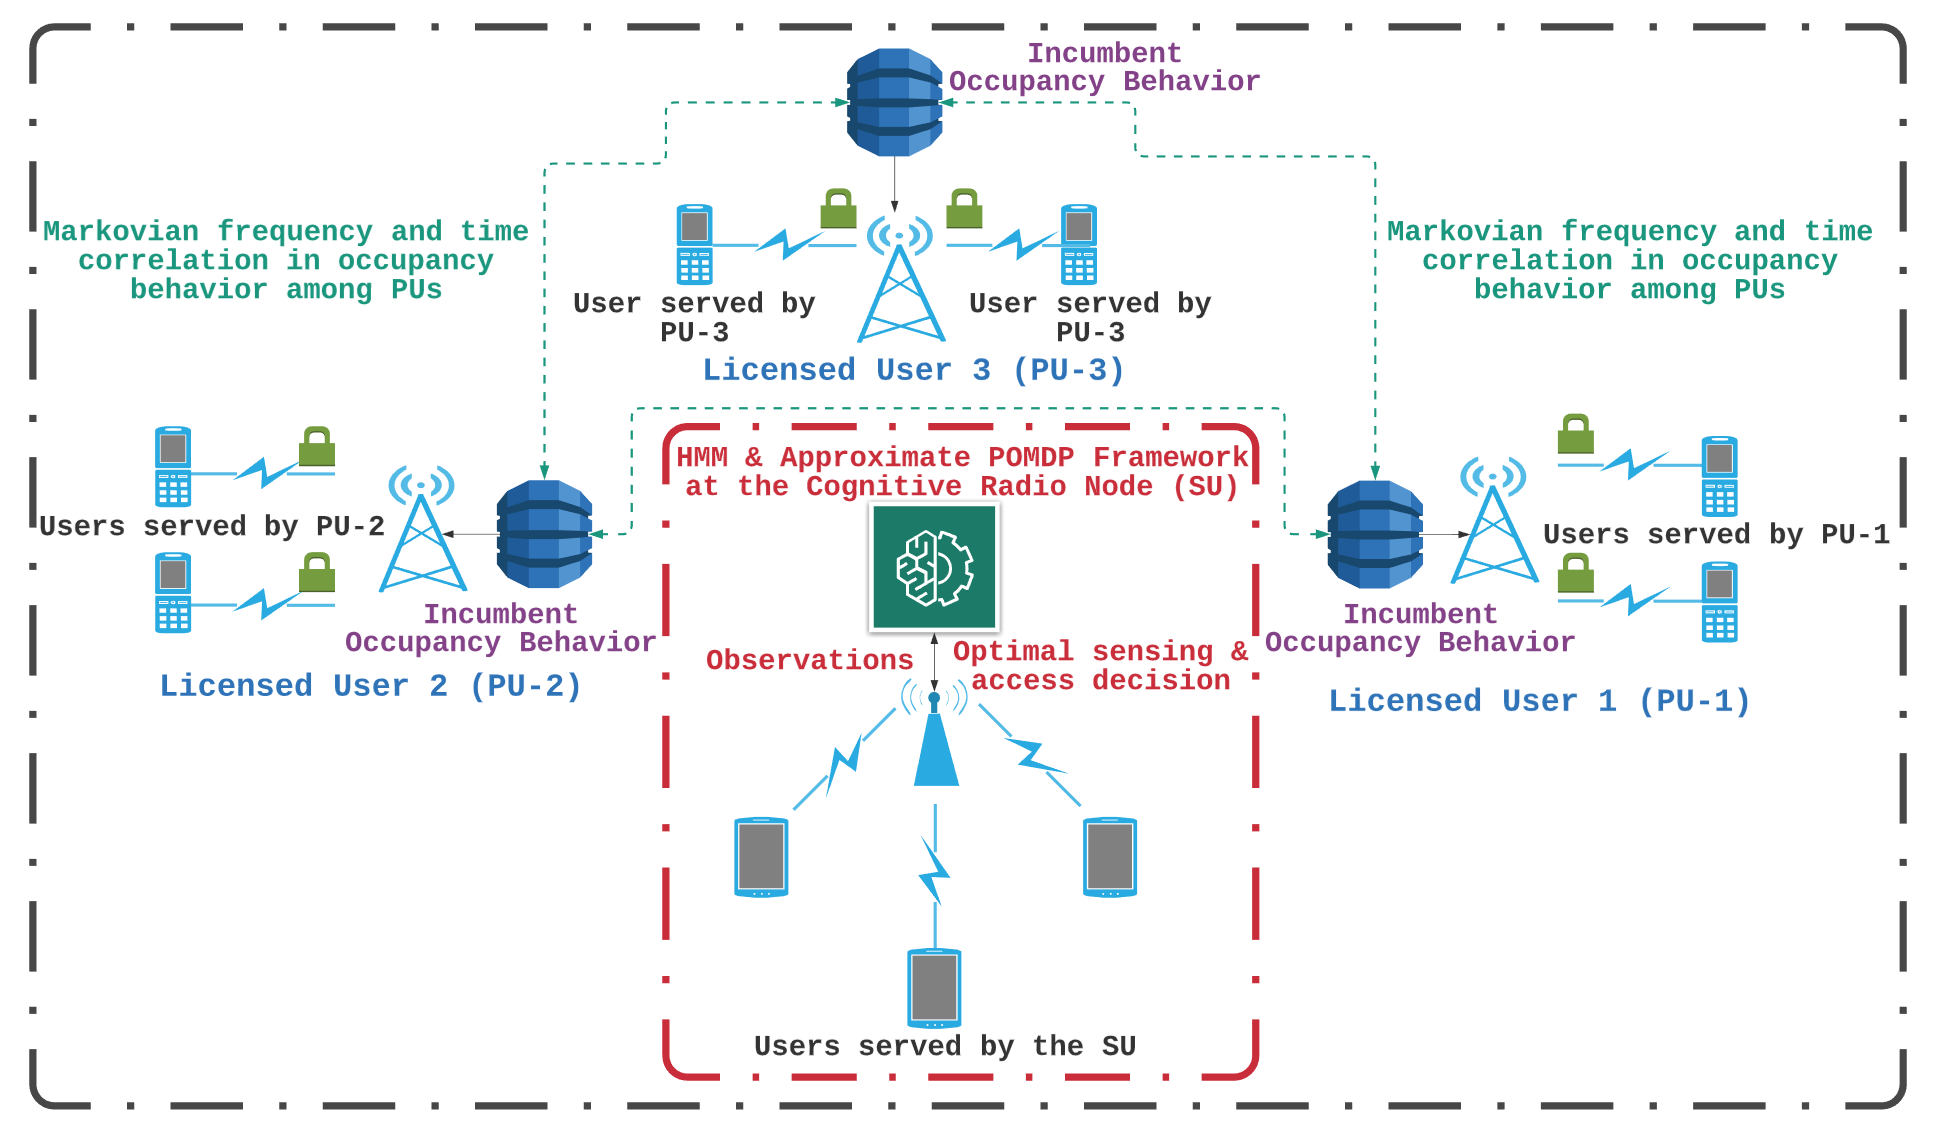
\includegraphics[width = 1.0\textwidth]{Minerva_System_Model.png}}
    \caption{The radio ecosystem under analysis: An exemplification of the system model detailed in Sec. \ref{I.I} with $J{=}3$, $K{=}18$, and $\kappa{=}3$.}
    \label{fig: A.0}
\end{figure}
A cognitive radio, referred to hereafter in this section as the Secondary User (SU), constitutes a spectrum-sensing is tasked with the objective of maximizing its throughput (to satisfy the imposed QoS requirements) while limiting interference with the priority or licensed users in the network, hereafter referred to in this section as the Primary Users (PUs). As discussed in Sec.  \ref{O}, these PUs (also known as incumbents) can either be military applications or commercial service providers who buy licenses from the FCC for access to the spectrum. We study a wireless radio environment in which the spectrum of interest has been discretized into $K$ channels of equal bandwidth $W$, with $J$ PUs and an SU trying to exploit portions of the spectrum left unused by these PUs, across time-slots and across frequencies\texttt{-{}-}as illustrated in Fig. \ref{fig: A.0}. The discretized wide-band signal received at the SU's spectrum sensor in time-slot $i$ can be described in the frequency domain as
\begin{equation}\label{1}
    Y_{k}(i)=\sum_{j{=}1}^{J}{H_{j,k}(i)X_{j,k}(i)+V_{k}(i)},
\end{equation}
where $X_{j,k}(i)$ represents the frequency domain signal of PU $j{\in}\{1,2,\dots,J\}$ in channel $k \in \{1,2,\dots,K\}$, with $X_{j,k}(i){=}0$, if PU $j$ is not transmitting over channel $k$ in time-slot $i$; $H_{j,k}(i)$ denotes the frequency domain channel between the SU and PU $j$; and $V_{k}(i){\sim}\mathcal{CN}(0,\sigma_{V}^{2})$ constitutes the zero-mean circularly symmetric additive complex Gaussian noise with variance $\sigma_{V}^{2}$, i.i.d across frequency and time, and independent of the channel $H$ and the PU signal $X$. Assuming an Orthogonal Frequency Division Multiple Access (OFDMA) strategy among the PUs with respect to the channels in this discretized spectrum, and letting $X_{k}(i){\triangleq}X_{j_{k,i},k}(i)$ and $H_{k}(i){\triangleq}H_{j_{k,i},k}(i)$, where subscript $j_{k,i}$ denotes the index of the PU that occupies channel $k$ in time-slot $i$, we can rewrite \eqref{1} as
\begin{equation}\label{2}
    Y_{k}(i)=H_{k}(i)X_{k}(i)+V_{k}(i),
\end{equation}
where $X_{k}(i){=}0$, if channel $k$ is not occupied by any PU in time-slot $i$, and $H_{j,k}(i) \sim \mathcal{CN}(0,\sigma_{H}^{2})$ constitutes the zero-mean circularly symmetric complex Gaussian random variable with variance $\sigma_{H}^{2}$, modeling the Rayleigh fading channel, i.i.d across frequency and time.
\subsection{Occupancy Correlation Structure}\label{I.II}
\begin{figure} [htb]
    \centerline{
    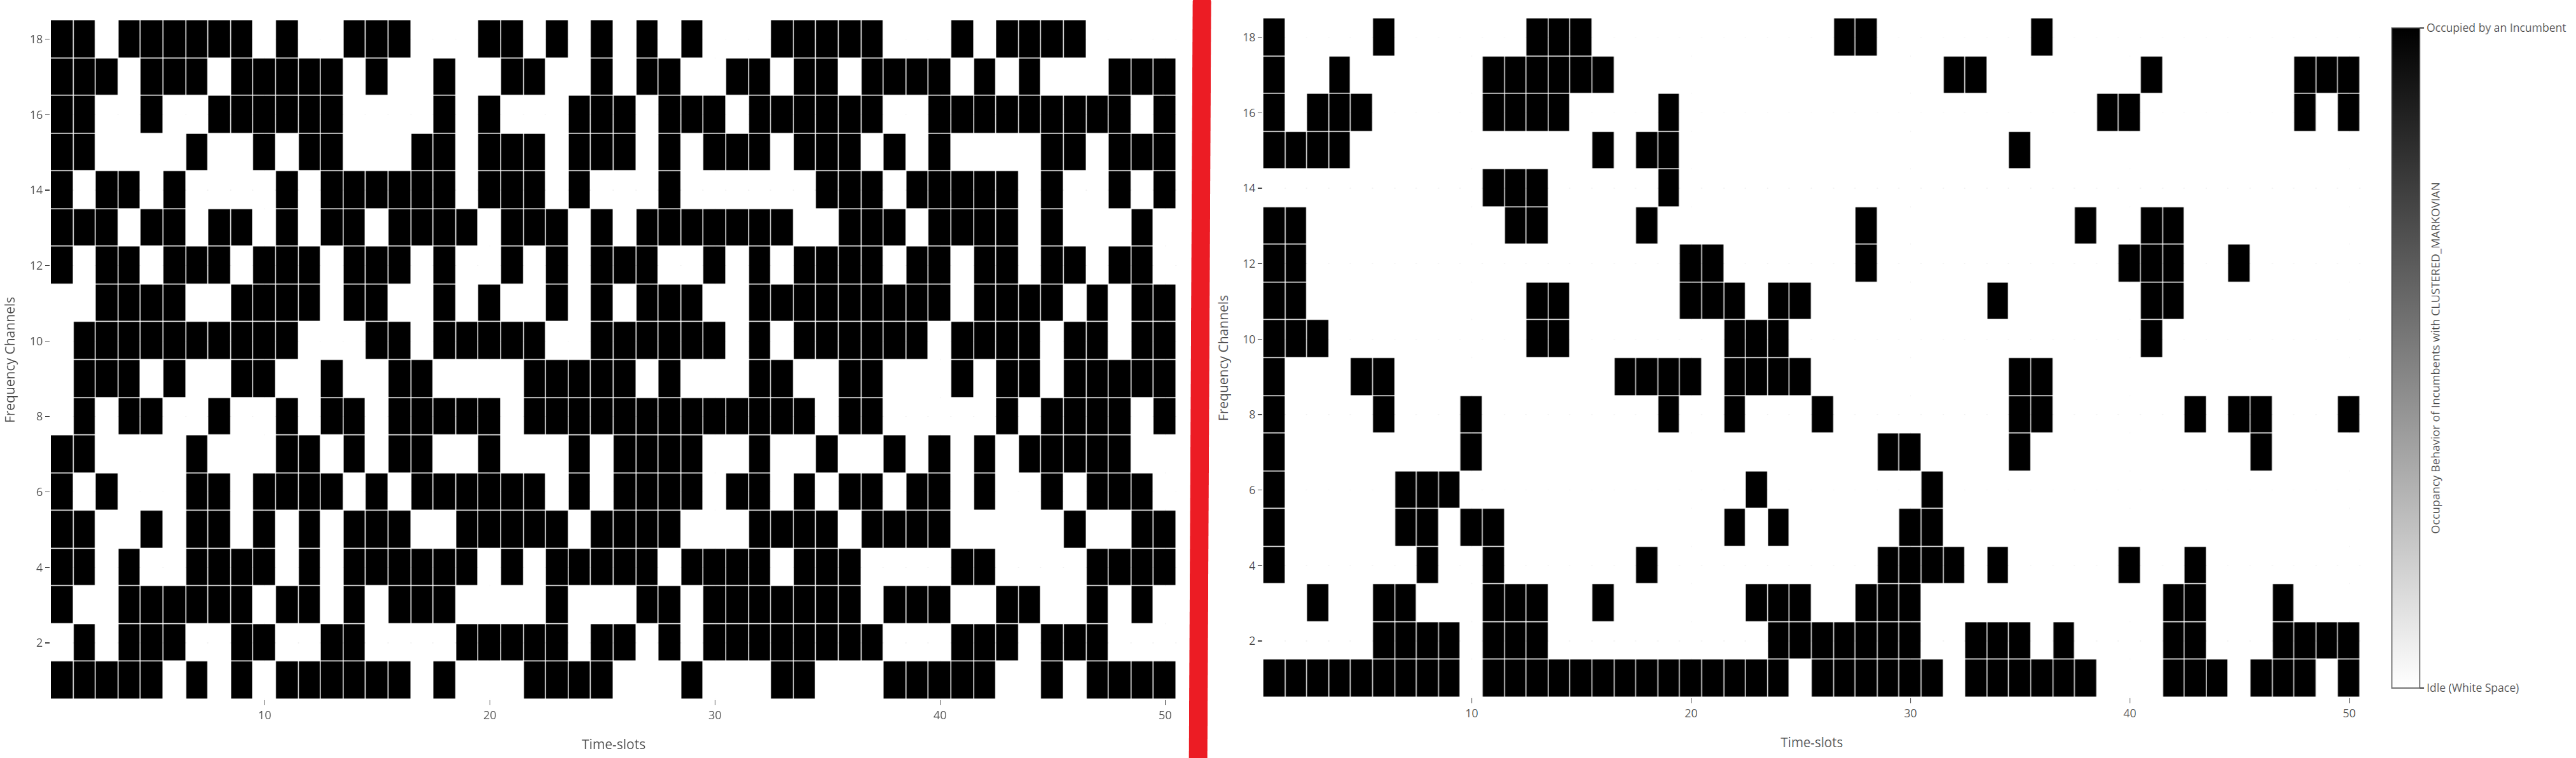
\includegraphics[width = 1.0\textwidth]{Minerva_Independent_Occupancy_Model.png}}
    \caption{The incumbent spectrum occupancy heat-map assuming independence across both frequency and time}
    \label{fig:A.1}
\end{figure}
\begin{figure} [htb]
    \centerline{
    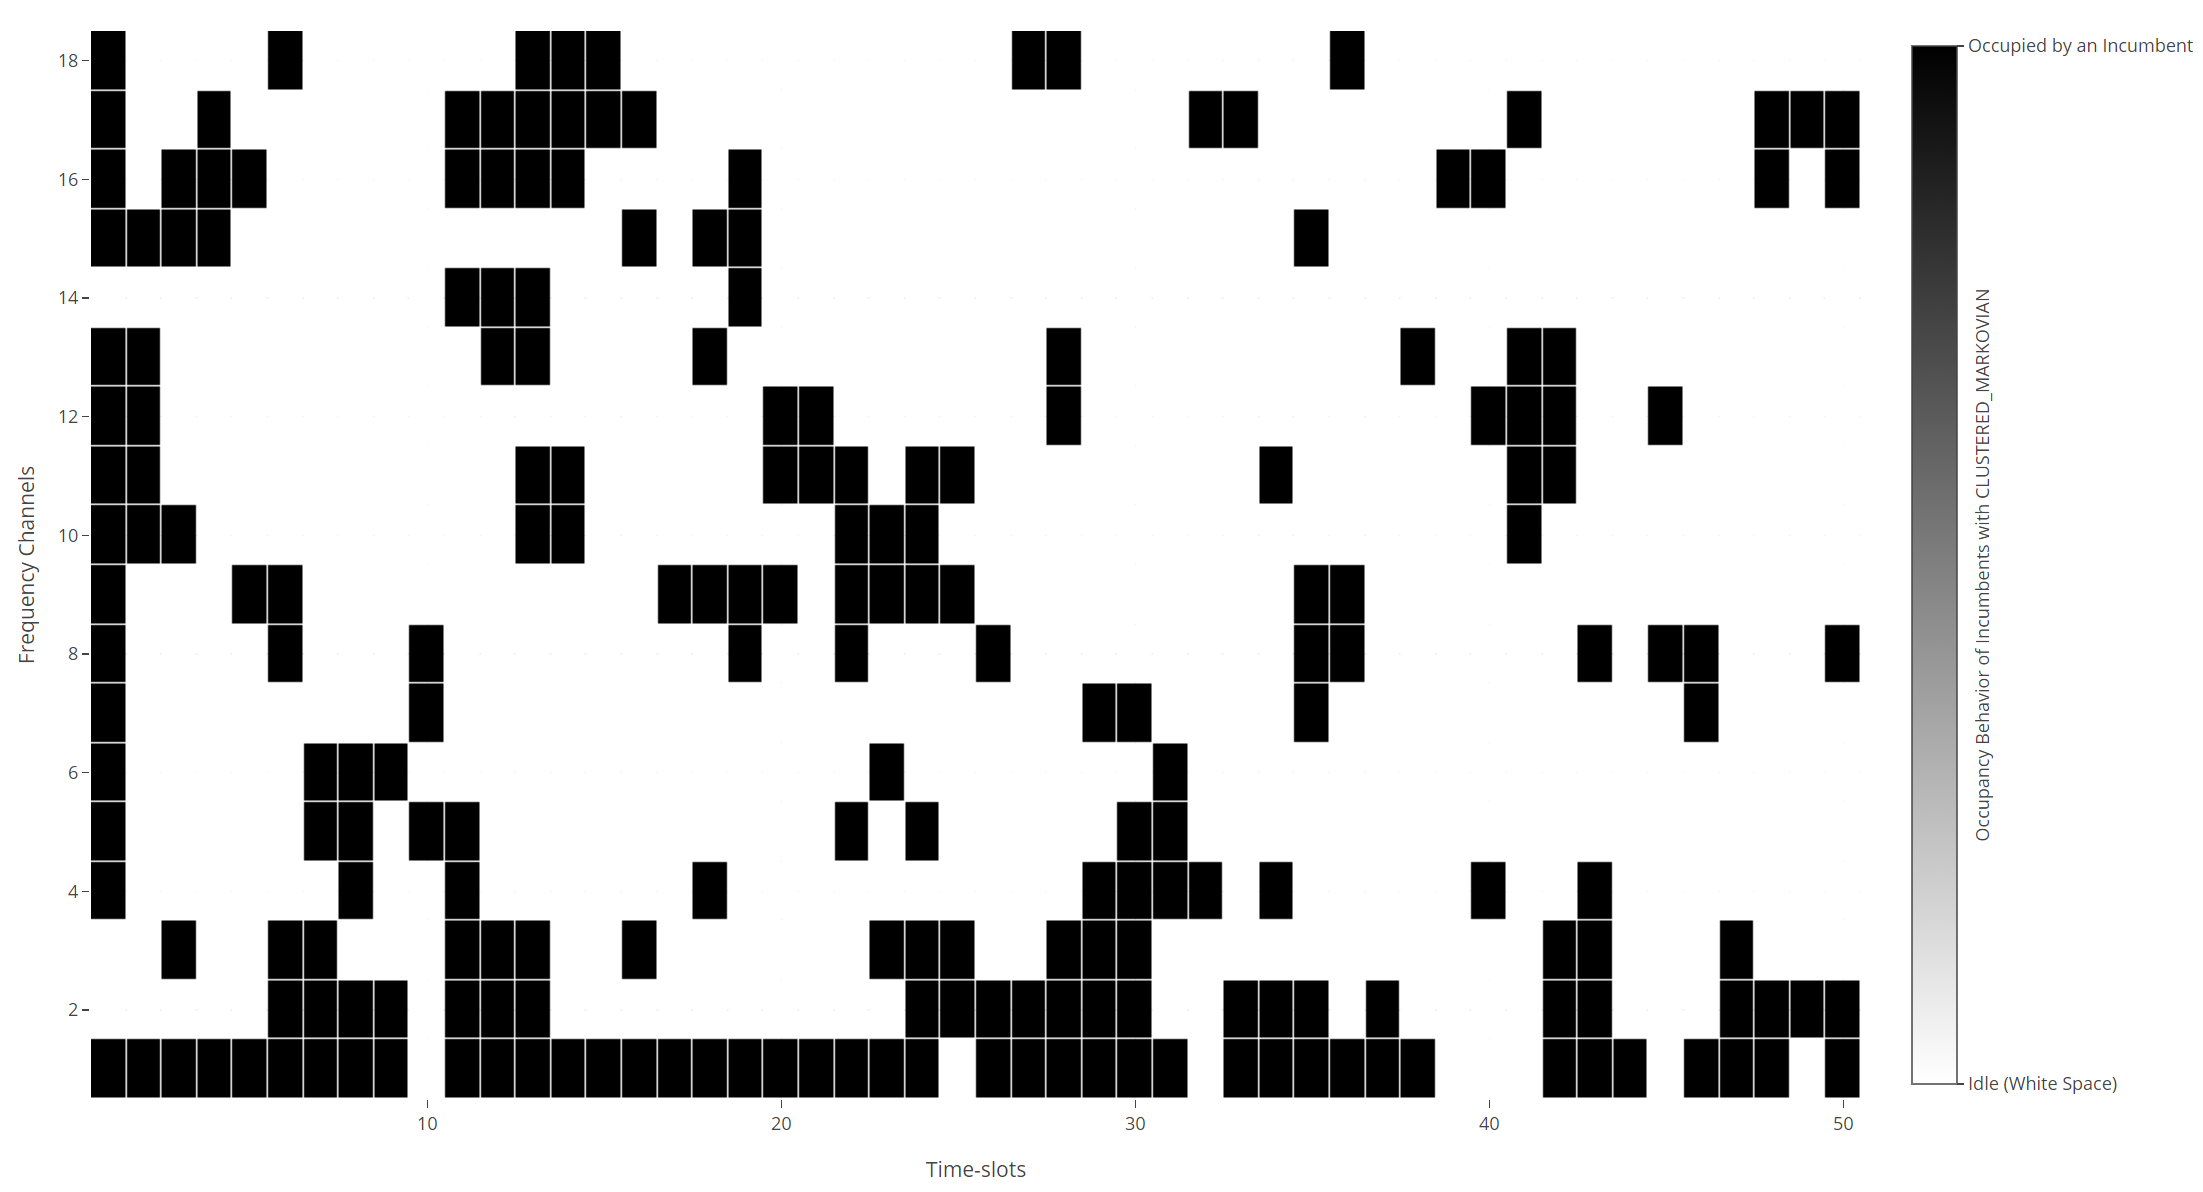
\includegraphics[width = 1.0\textwidth]{Minerva_Markovian_Occupancy_Model.png}}
    \caption{The incumbent spectrum occupancy heat-map assuming a time-frequency correlation structure}
    \label{fig:A.2}
\end{figure}
\begin{figure} [htb]
    \centerline{
    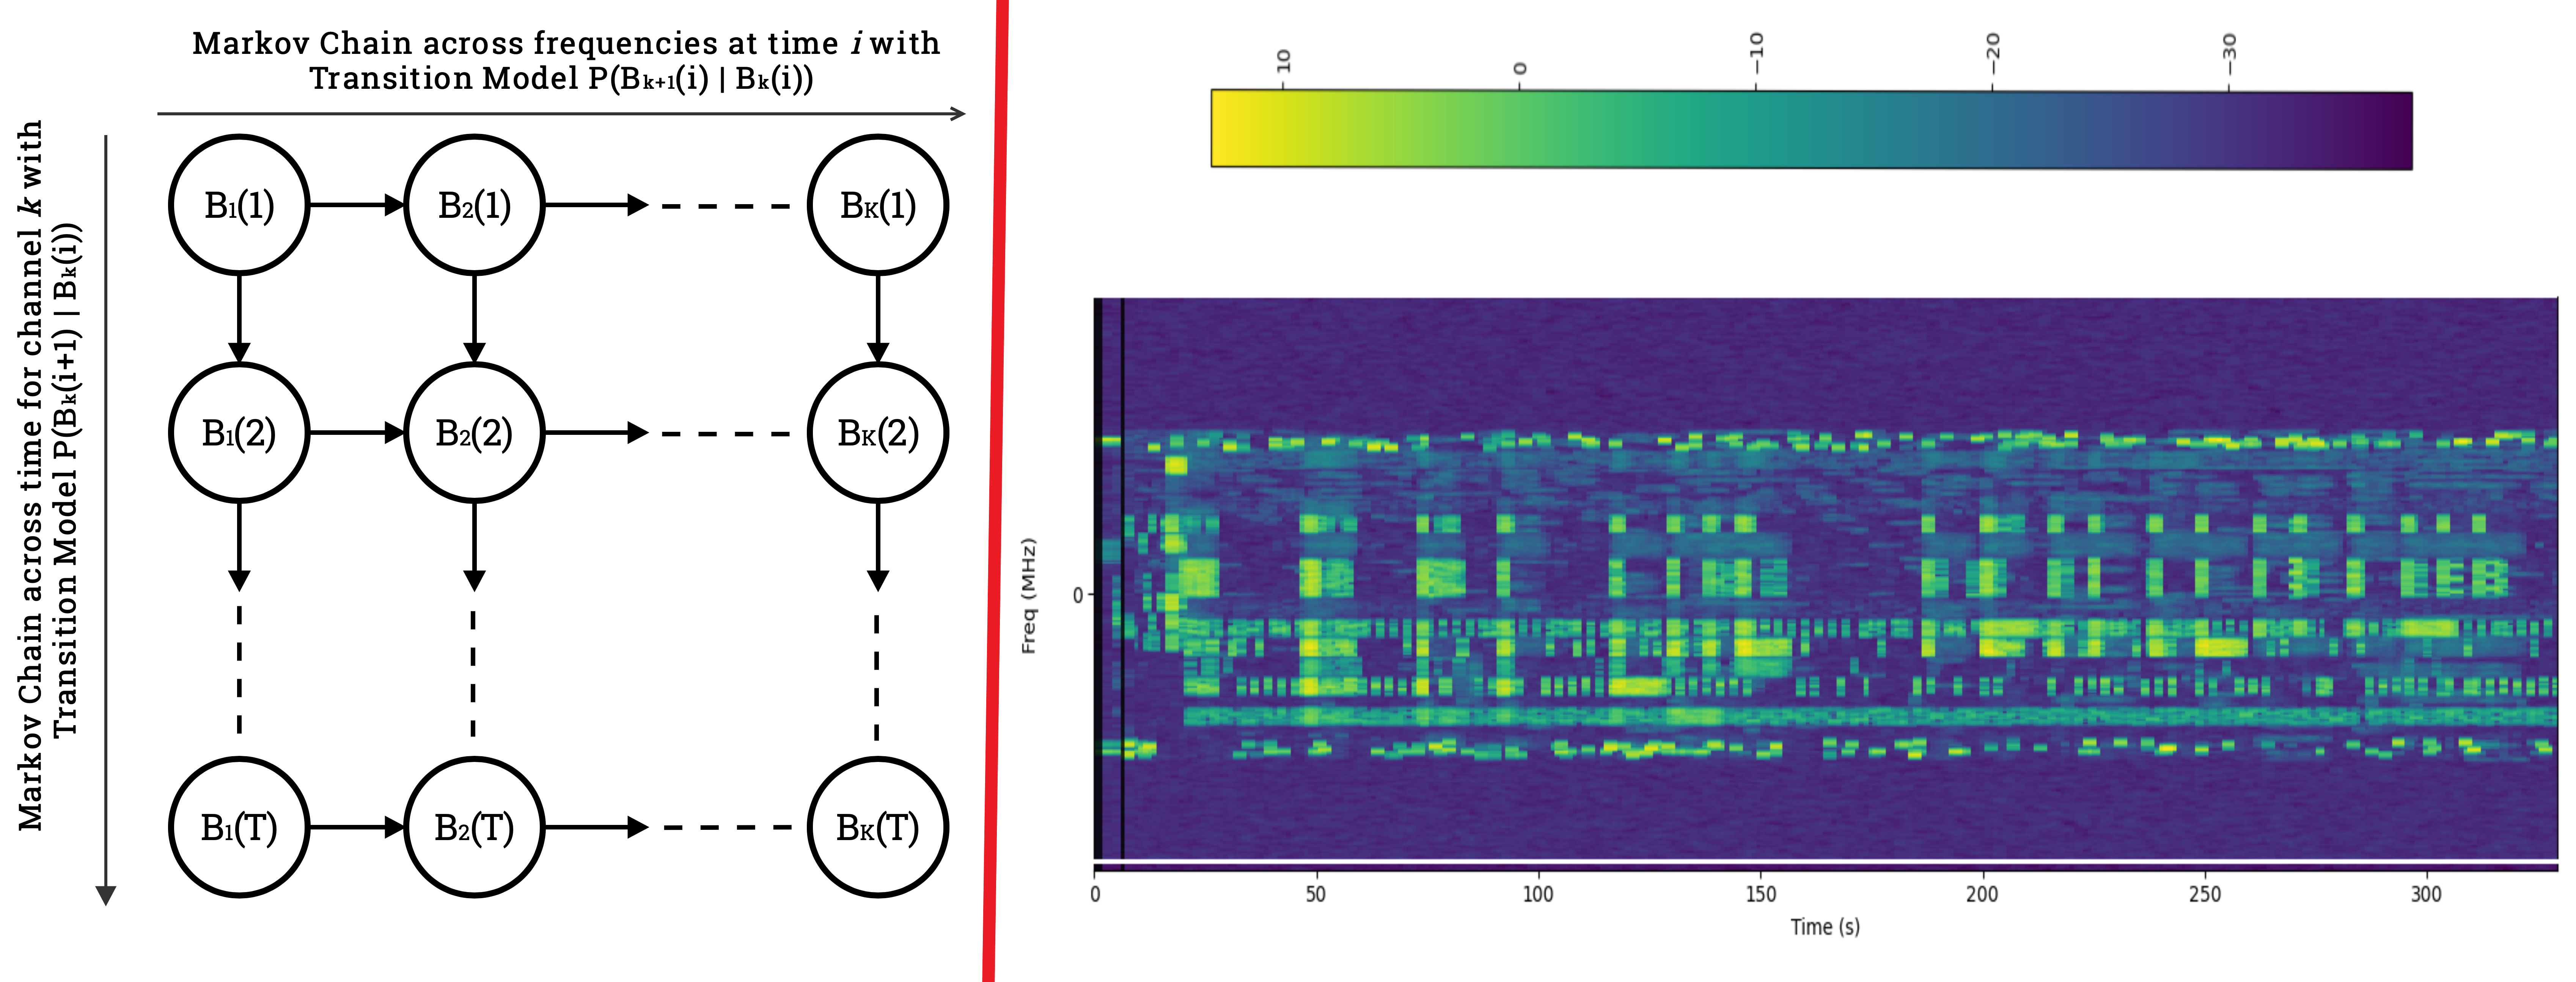
\includegraphics[width = 1.0\textwidth]{MarkovChainsVisualization.png}}
    \caption{The visualization of the incumbent occupancy time-frequency correlation structure as two dependent Markov chains: one across time and the other across frequencies}
    \label{fig:A.3}
\end{figure}
The frequency domain signal of the PU occupying channel $k$ in time-slot $i$ is modeled as
\begin{equation}\label{3}
    X_{k}(i)=\sqrt{P_{T}}B_{k}(i)S_{k}(i),
\end{equation}
where $P_{T}$ denotes the transmission power of the occupant PU (we assume that all the PUs exhibit some kind of power control mechanisms in their PHY, and therefore have the same transmission power $P_{T}$), $B_{k}(i)$ represents the binary channel occupancy variable, i.e., $B_{k}(i){=}1$, if channel $k$ is occupied by a PU in time-slot $i$, $B_{k}(i){=}0$, otherwise, and $S_{k}(i)$ denotes the transmitted symbol. $S_{k}(i)$ can be modeled as a constant amplitude signal, i.e., $|S_{k}(i)|{=}1$, i.i.d across frequency and time; if however, $S_{k}(i)$ is not a constant amplitude signal, we write $H_{k}(i)X_{k}(i)$ as $\sqrt{P_{T}}B_{k}(i)H_{k}(i)S_{k}(i)$, where $H_{k}(i)S_{k}(i)$ can be approximated as a zero-mean complex Gaussian random variable with variance $\sigma_{H}^{2}\mathbb{E}[|S_{k}|^{2}]$, without any modifications to the subsequent analysis \cite{WCL:paper}. The spectrum occupancy state in time-slot $i$ can be written as
\begin{equation}\label{4}
    \vec{B}(i)=[B_{1}(i),B_{2}(i),B_{3}(i),\dots,B_{K}(i)]^{\intercal},
\end{equation}
where $\vec{B}(i){\in}\{0,1\}^{K}$. There exists a time-frequency correlation structure in the occupancy behavior of the PUs in the network because a PU usually occupies adjacent channels for prolonged periods of time, i.e., the incumbents usually restrict their transmissions to certain parts of the spectrum, occupying a set of adjacent bands, and exhibit temporal patterns in their occupancy of these bands, with the temporal patterns governed by the operational periodicity of military users or by the prolonged usage by licensed service providers \cite{WCL:12}. We decompose this time-frequency correlation structure as follows \cite{WCL:paper}: we model the temporal correlation in incumbent occupancy behavior as a Markov process described by
\begin{equation}\label{5}
    \mathbb{P}(\vec{B}(i+1)|\vec{B}(j),\forall j \leq i)=\mathbb{P}(\vec{B}(i+1)|\vec{B}(i)),
\end{equation}
and we couple this model with the another Markov chain across the frequency bands to capture the frequency correlation in incumbent occupancy behavior, to get the final correlation structure as
\begin{equation}\label{6}
    \mathbb{P}(\vec{B}(i+1)|\vec{B}(i))=\mathbb{P}(B_{1}(i+1)|B_{1}(i))\prod_{k=2}^{K}\mathbb{P}(B_{k}(i+1)|B_{k-1}(i+1),B_{k}(i)).
\end{equation}
In other words, we can describe this Markovian time-frequency correlation as follows: the occupancy of frequency band $k$ in time-slot $i+1$ depends on the occupancy of the adjacent frequency band $k-1$ in the same time-slot $i+1$, and the occupancy of the same frequency band $k$ in the previous time-slot $i$. We parameterize this two-chain Markovian correlation structure by
\begin{equation}\label{7}
    \begin{aligned}
        \vec{\theta}&=[\vec{p}\ \vec{q}]^{\intercal},\ \text{where}\\
        \vec{p}&=[p_{uv}=\mathbb{P}(B_{k}(i+1)=1|B_{k-1}(i+1)=u,B_{k}(i)=v):u,v \in \{0,1\}]^{\intercal},\ \text{and}\\
        \vec{q}&=[q_{w}=\mathbb{P}(B_{1}(i+1)=1|B_{1}(i)=w):w \in \{0,1\}]^{\intercal}.
    \end{aligned}
\end{equation}
This vector $\vec{\theta}$, parameterizes the transition model of our POMDP formulation described in Section \ref{I.IV}, and is estimated by an HMM-specific Expectation Maximization (EM) algorithm, i.e., the Baum-Welch algorithm, which is the solution to the framed MLE problem, all of which is detailed in Section \ref{II.I}.

Fig. \ref{fig:A.1} illustrates the spectrum occupancy heat-map, assuming independence in occupancy behavior across both frequency and time, while Fig. \ref{fig:A.2} depicts the spectrum occupancy heat-map, assuming a time-frequency correlation structure in incumbent occupancy behavior, with $\vec{p}{=}[p_{00}{=}0.1,p_{01}{=}0.3,p_{10}{=}0.3,p_{11}{=}0.7]^{\intercal}$ and $\vec{q}=[q_{0}{=}0.3,q_{1}{=}0.8]^{\intercal}$. The time-frequency correlation structure underlying the occupancy behavior of PUs in the network, as described by \eqref{6}, can be illustrated as two dependent Markov chains: one across time and the other across frequencies, as shown in Fig. \ref{fig:A.3}.
\subsection{Channel Sensing Model}\label{I.III}
Equipped with a spectrum sensor, the SU detects white spaces and accesses them to deliver its network flows. Owing to physical design limitations\texttt{-{}-}specifically, the restriction on the number of channels that can sensed by the SU's spectrum sensor in any given time-slot, primarily due to concerns about energy-efficiency and sensing/data aggregation times \cite{WCL:3}, the SU can sense a maximum of $\kappa$ spectrum bands in a time-slot, with $1{\leq}\kappa{\leq}K$. In a specific time-slot $i$, the SU senses all the channels in the set $\mathcal{K}_{i}{\subseteq}\{1,2,\dots,K\}$, with the sensing limitation imposed as $|\mathcal{K}_{i}|{\leq}\kappa$. The solution to the spectrum sensing problem is to determine an optimal set of channels sensed by the SU in any time-slot $i$, and this optimal set is dictated by the optimal policy derived from the POMDP formulation via the PERSEUS algorithm detailed in Section \ref{II.II}. The solution to the access problem hinges on the optimal sensing policy, i.e., based on the ``best-possible" spectrum occupancy picture painted by the optimal sensing action in a time-slot $i$, the SU accesses all the channels it deems to be idle\texttt{-{}-}more details on this access strategy are discussed in Section \ref{I.IV}. After sensing the channels listed in $\mathcal{K}_{i}$, governed by the sensing policy, the obtained observation vector $\vec{Y}(i){=}[Y_{k}(i)]_{k{\in}\mathcal{K}_{i}}]$, where $Y_{k}(i)$ is described in \eqref{2} \cite{WCL:paper}.

In statistics, Hidden Markov Models (HMMs) are used to describe systems modeled by Markov processes, with the actual system states ``hidden" behind the observed noisy measurements of these states. Along these lines, constructing an HMM for our problem, the linear, additive, Gaussian noise in the observation model described in Section \ref{I.I}, introduces uncertainty into the sensing process\texttt{-{}-}the true occupancy states of the frequency bands in time-slot $i$, i.e., $\vec{B}(i)$, represent the actual states of the model, while the observations at the SU's spectrum sensor, i.e., $\vec{Y}(i)$, represent the noisy observations of these true occupancy states. The observation vector in time-slot $i$, $\vec{Y}(i)$, given the occupancy vector in that time-slot, $\vec{B}(i)$, has a Probability Density Function (PDF) described by
\begin{equation}\label{8}
    f(\vec{Y}(i)|\vec{B}(i),\mathcal{K}_{i})=\prod_{k=1}^{K}f(Y_{k}(i)|B_{k}(i)),
\end{equation}
due to the i.i.d assumptions of the noise, $V_{k}(i)$, the transmitted symbols, $S_{k}(i)$, and the Rayleigh fading variables $H_{k}(i)$, across channels, given the occupancy state vector, as discussed in Section \ref{I.I}. Additionally, we can infer from \eqref{2} that
\begin{equation}\label{9}
    Y_{k}(i)|B_{k}(i)\sim\mathcal{CN}(0,\sigma_{H}^{2}P_{T}B_{k}(i)+\sigma_{V}^{2}).
\end{equation}
\subsection{POMDP Formulation}\label{I.IV}
Partially Observable Markov Decision Processes (POMDPs) are employed in modeling the repeated, sequential interactions of an agent\texttt{-{}-}tasked with maximizing its reward, subject to the problem at hand\texttt{-{}-}with a stochastic environment, wherein the limited observational capacity of the agent and/or the observation noise, creates partial observability vis-\`{a}-vis the underlying states of the environment. Modeling the spectrum sensing process at the SU as a POMDP, we find that, as expected, the partial observability caused by the sensing restrictions and a noisy observation model, result in an increased level of uncertainty regarding the exact effect of executing a spectrum access action on the radio environment \cite{WCL:paper}. Our POMDP formulation, represented by the 5-tuple $(\mathcal{B},\mathcal{A},\mathcal{Y},\mathbf{A},\mathbf{M})$, features the state space of the underlying MDP, denoted by $\mathcal{B}{\equiv}\{0,1\}^{K}$, which is given by all possible realizations of the occupancy vector $\vec{B}$; the action space of the SU, denoted by $\mathcal{A}$, which is described by all possible combinations in which $1{\leq}\kappa{\leq}K$ channels are chosen to be sensed in a time-slot (discussed in Section \ref{I.III}; the observation space, denoted by $\mathcal{Y}$, which is discussed in Section \ref{I.I}; the transition model of the underlying MDP, denoted by $\mathbf{A}$, which is discussed in Section \ref{I.II}; and the observation model (also known as the emission model), denoted by $\mathbf{Y}$, which is described by \eqref{8} and \eqref{9}.

Prior to gathering the occupancy information in time-slot $i$, based on the measurements obtained by the SU's spectrum sensor up to, but not including, time-slot $i$, the POMDP state is described by the prior belief, denoted by $\beta_{i}$, which describes the probability distribution of the underlying MDP state, i.e., $\vec{B}(i)$. Given this prior belief $\beta_{i}$, based on the SU's sensing policy, the SU chooses a sensing action, i.e., $\pi(\beta_{i})=\mathcal{K}_{i}{\in}\mathcal{A}$, wherein as detailed in Section \ref{I.III}, the SU senses the frequency bands corresponding to the channel indices in the set $\mathcal{K}(i)$, and this observation vector $[Y_{k}(i)]_{k{\in}\mathcal{K}_{i}}{\in}\mathcal{Y}$, and updates its belief of the underlying MDP state $\vec{B}(i)$ to obtain its posterior belief, which is written as
\begin{equation}\label{10}
    \begin{aligned}
        \hat{\beta}_{i}(\vec{B}')&=\mathbb{P}(\vec{B}(i)=\vec{B}'|\beta_{i},\mathcal{K}_{i},[Y_{k}(i)]_{k{\in}\mathcal{K}_{i}})\\
        &=\frac{\mathbb{P}([Y_{k}(i)]_{k{\in}\mathcal{K}_{i}}|\vec{B}',\mathcal{K}_{i})\beta(\vec{B}')}{\sum_{\vec{B}'' \in \{0,1\}^{K}}\mathbb{P}([Y_{k}(i)]_{k{\in}\mathcal{K}_{i}}|\vec{B}'',\mathcal{K}_{i})\beta_{i}(\vec{B}'')}.
    \end{aligned}
\end{equation}
After channel sensing is performed by the SU's spectrum sensor, according to the sensing policy, using the posterior belief described in \eqref{10}, channel access decisions have to be made: the underlying MDP state $\vec{B}(i)$ is estimated as
\begin{equation}\label{11}
    \vec{\phi}(\hat{\beta}_{i})=\argmax_{\vec{B} \in \mathcal{B}}\hat{\beta}_{i}(\vec{B}),
\end{equation}
following which, if $\phi_{k}(i){=}1$, which implies that the SU estimated channel $k$ to be occupied by a PU in this time-slot $i$, and hence leaves it untouched, while if $\phi_{k}(i){=}0$, the SU accesses this ``estimated idle" channel $k$ in time-slot $i$ to deliver its network flows. Upon executing an access decision based on the Maximum-A-Posteriori (MAP) estimation procedure laid down in \eqref{11}, i.e., in time-slot $i$, after accessing all the channels with $\phi_{k}(i){=}0$, the SU receives a reward from the radio environment, denoted by $R(\vec{B}(i),\hat{\beta}_{i})$, dictated by the number of truly idle frequency bands accessed by the SU, which accounts for the SU throughput maximization aspect of its objective, and a penalty ($\lambda{>}0$) for the number of incumbent occupied channels that were incorrectly accessed by the SU, which accounts for the aspect of its objective that involves minimizing the interference caused to PUs in the network \cite{WCL:paper}. Mathematically, this reward metric is described as
\begin{equation}\label{12}
    R(\vec{B}(i),\hat{\beta}_{i})=\sum_{k=1}^{K}(1-B_{k}(i))(1-\phi_{k}(i))-\lambda B_{k}(i)(1-\phi_{k}(i)).
\end{equation}
Ensuing the determination of the reward for its access decision from the radio environment, the SU computes the prior belief for the next time-slot $i+1$ as
\begin{equation}\label{13}
    \beta_{i+1}(\vec{B}'')=\sum_{\vec{B}'}\mathbb{P}(\vec{B}(i+1)=\vec{B}''|\vec{B}(i)=\vec{B}')\hat{\beta}(\vec{B}').
\end{equation}
Let
\begin{equation}\label{14}
    \hat{\beta}_{i}=\hat{\mathbb{B}}(\beta_{i},\mathcal{K}_{i},\vec{Y}(i))
\end{equation}
denote the function that maps the prior belief $\beta_{i}$ to the posterior belief $\hat{\beta}_{i}$ in time-slot $i$, and let
\begin{equation}\label{15}
    \beta_{i+1}=\mathbb{B}(\hat{\beta}_{i})
\end{equation}
denote the function that maps the posterior belief $\hat{\beta}_{i}$ in time-slot $i$ to the prior belief $\beta_{i+1}$ in time-slot $i+1$ \cite{WCL:paper}. The objective of the SU is to determine the optimal spectrum sensing policy (based on which the access decisions are made in the corresponding time-slots) to maximize its infinite-horizon discounted reward, i.e.,
\begin{equation}\label{16}
    \pi^{*}=\argmax_{\pi}V^{\pi}(\beta),
\end{equation}
where
\begin{equation}\label{17}
    V^{\pi}(\beta)=\mathbb{E}_{\pi}\left[\sum_{i=1}^{\infty}\gamma^{i}R(\vec{B}(i),\hat{\beta}_{i})\Big{|}\beta_{0}=\beta\right],
\end{equation}
where $0{<}\gamma{<}1$ is the discount factor, $\beta_{0}{=}\beta$ is the initial belief such that the value function $V^{\pi}(\beta)$ is evaluated from this starting belief, and $\hat{\beta}_{i}$ is the posterior belief induced by the policy $\mathcal{K}_{i}{=}\pi(\beta_{i})$ and the observation vector $[Y_{k}(i)]_{k{\in}\mathcal{K}_{i}}$ via the formulation $\hat{\beta}_{i}{=}\hat{\mathbb{B}}(\beta_{i},\mathcal{K}_{i}{=}\pi(\beta_{i}),[Y_{k}(i)]_{k{\in}\mathcal{K}_{i}})$ \cite{WCL:paper}. The Bellman operator, denoted by $\mathcal{H}$, employed in the Bellman optimality equation, $V^{*}{=}\mathcal{H}(V^{*})$, is defined at iteration $t+1$ as, $\forall{\beta}$
\begin{equation}\label{18}
    \begin{aligned}
        V_{t+1}&=\mathcal{H}(V_{t})\\
        &=\max_{\mathcal{K} \in \mathcal{A}}\sum_{\vec{B} \in \mathcal{B}}\beta(\vec{B})\mathbb{E}_{[Y_{k}]_{k \in \mathcal{K}}|\vec{B},\mathcal{K}}\left[R(\vec{B},\hat{\mathbb{B}}(\beta,\mathcal{K},[Y_{k}]_{k \in \mathcal{K}}))+\gamma V_{t}(\mathbb{B}(\hat{\mathbb{B}}(\beta,\mathcal{K},[Y_{k}]_{k \in \mathcal{K}}))\right].
    \end{aligned}
\end{equation}
\begin{figure} [htb]
    \centerline{
    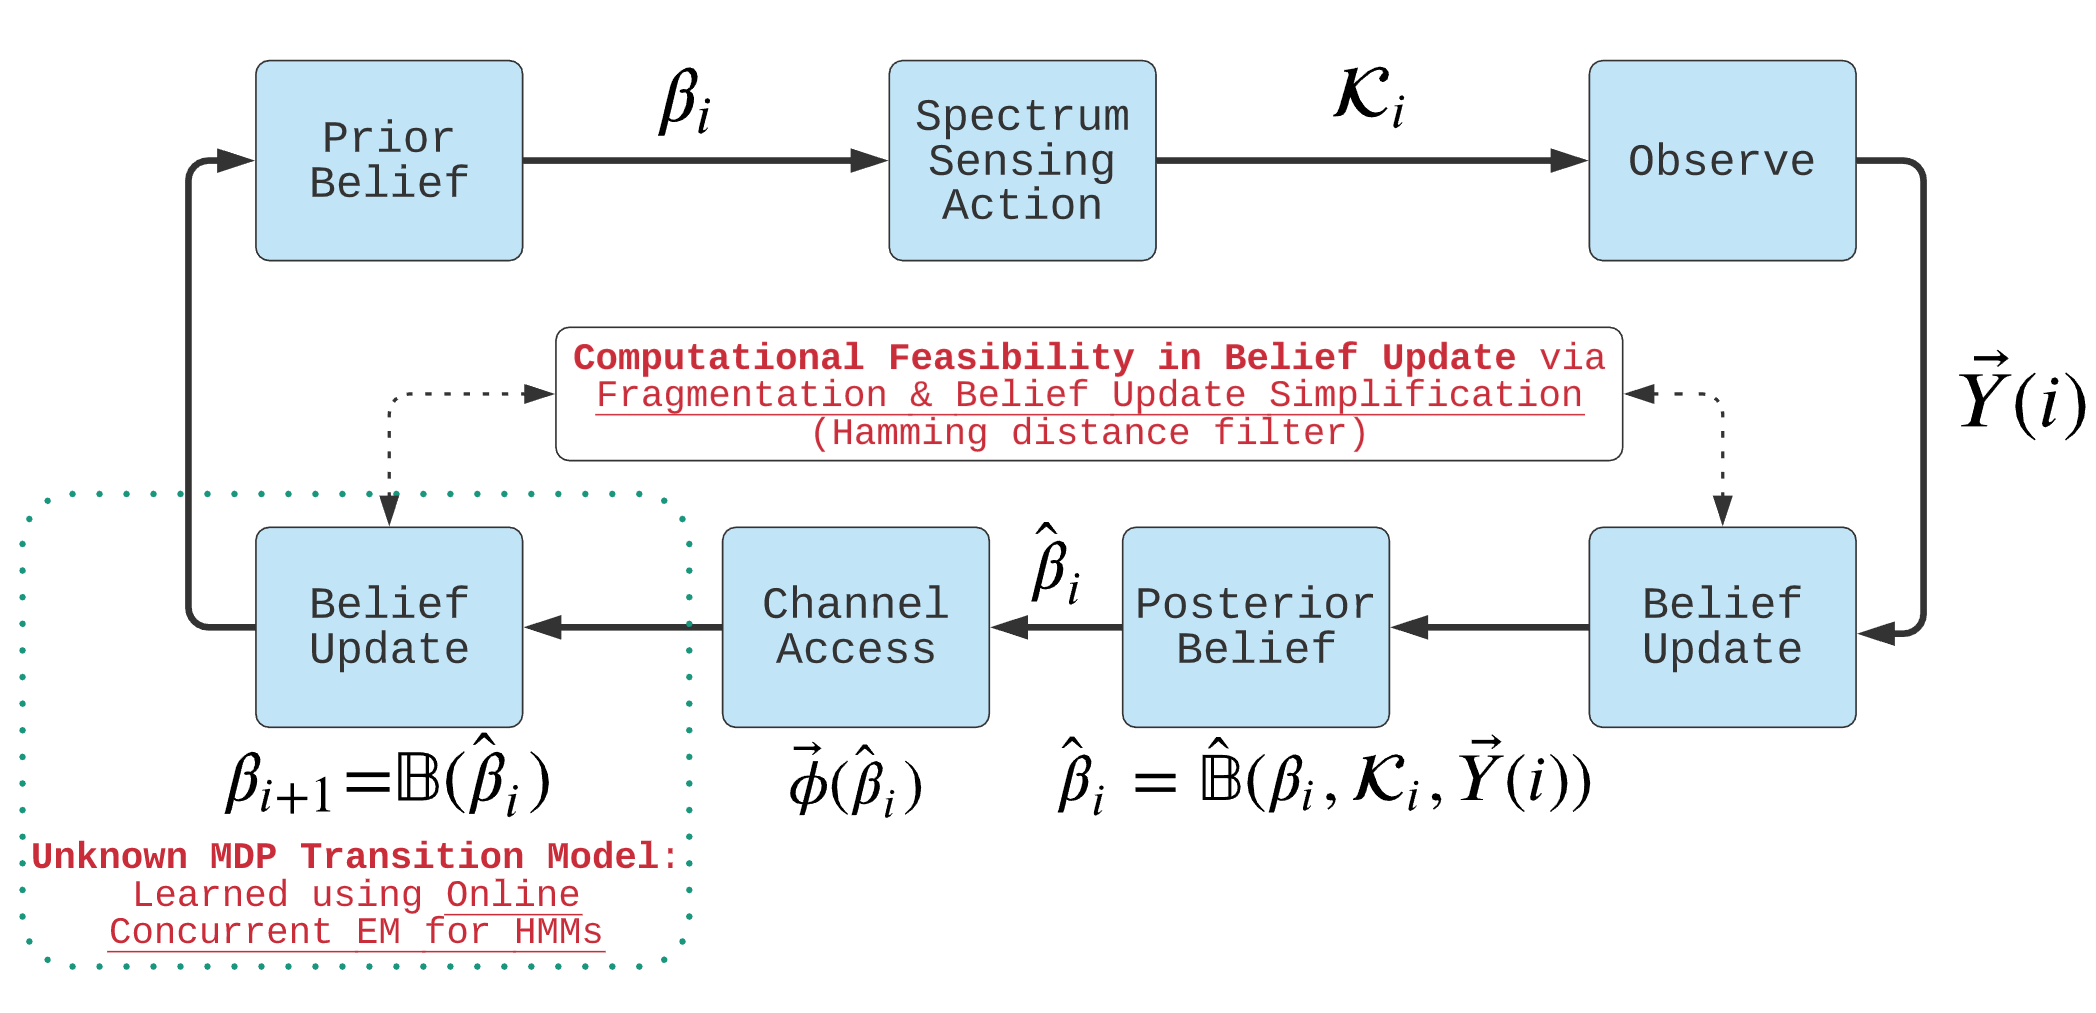
\includegraphics[width = 1.0\textwidth]{Minerva_POMDP_Model.png}}
    \caption{The POMDP process flow as discussed in Sec. \ref{I.IV}}
    \label{fig: A.add-1}
\end{figure}
By employing value iteration algorithms, \eqref{18} can be solved iteratively until convergence to a fixed point that corresponds to the optimal sensing policy. However, this direct approach results in complications associated with the lack of prior knowledge about the incumbent occupancy time-frequency correlation structure that defines the transition model of the underlying MDP, and the computational infeasibility of the approach\texttt{-{}-}as the number of channels in the discretized spectrum of interest increases, the number of states of the underlying MDP scales exponentially, resulting in a high-dimensional belief space, which makes the approach intractable \cite{WCL:paper}. An illustration of the POMDP formulation is provided in Fig. \ref{fig: A.add-1}.

We solve the problem of intractability of the POMDP for large state and action spaces by employing a randomized, point-based, approximate value iteration algorithm known as PERSEUS \cite{WCL:13} to solve for the optimal sensing policy, while an online parameter estimator embedded into PERSEUS allows us to solve the problem of transition model ignorance. Both these algorithms are detailed in Section \ref{II}.
\section{Proposed Solution: The Algorithms}\label{II}
\subsection{Occupancy Correlation Structure Estimation}\label{II.I}
Practical implementations of the MAC layer of the cognitive radio's network protocol stack involve solving for the optimal sensing and access policy, without having any prior information about the time-frequency correlation structure underlying the occupancy behavior of the incumbents in the network \cite{WCL:paper}. This correlation structure, as discussed earlier, can be leveraged to improve the occupancy state estimation accuracy, which in turn facilitates higher SU network throughput with lower PU interference. In this regard, in this section, we propose a parameter estimator algorithm that learns this correlation structure over time\texttt{-{}-}with the learned correlation structure iteratively fed into the POMDP optimal policy solver (i.e., PERSEUS), in order to enable a concurrent framework that minimizes the amount of computational resources (time, memory, processing power) required to obtain the optimal policy, which is especially crucial in non-stationary settings.

Let $\tau$ refer to the learning period of the parameter estimation algorithm: this can be equal to the entire duration of the SU's interaction with the radio environment while solving for the optimal policy, implying concurrent model learning facilitated by a publisher-subscriber software architecture and multi-threading features\texttt{-{}-}in a time-slot, the diverse, sparse observations made by the SU as a part of the PERSEUS thread's exploration period are concatenated into a complete observation vector over repeated iterations (we assume the dynamics of the PU occupancy over the time-slots are slower than the time needed for these observations and their subsequent concatenation) and injected into the EM thread, which estimates the transition probabilities in that iteration (which is synchronized with the PERSEUS thread's time-slot dynamics in order to have these two threads operate on the same time-scale) and publishes them, with the PERSEUS thread using the most current published estimates in its operation; or it can  be equal to an initial learning period that has been set aside exclusively for the SU to estimate the underlying MDP's transition model\texttt{-{}-}after which the PERSEUS algorithm is initiated, employing these final estimated (converged) transition probabilities. Defining $\mathbf{B}{=}[\vec{B}(i)]_{i{=}1}^{\tau}$ as the sequence of states encountered by the SU in time-slots $i{=}1$ to $i{=}\tau$, and $\mathbf{Y}{=}[\vec{Y}(i)]_{i{=}1}^{\tau}$ as the sequence of observations made at the SU's spectrum sensor $i{=}1$ to $i{=}\tau$, having a one-to-one correspondence with the elements of $[\vec{B}]_{i{=}}^{\tau}$, we formulate the Maximum Likelihood Estimation (MLE) problem to estimate the vector $\vec{\theta}$ that parameterizes the PU occupancy time-frequency correlation structure (detailed in Section \ref{I.II}) as follows:
\begin{equation}\label{19}
    \vec{\theta}^{*}=\argmax_{\vec{\theta}}\log{\left(\sum_{\mathbf{B}}\mathbb{P}(\mathbf{B},\mathbf{Y}|\vec{\theta})\right)}.
\end{equation}
Solving this MLE formulation using the Expectation-Maximization algorithm \cite{WCL:14} for HMMs, i.e., the Baum-Welch algorithm, the algorithm boils down to two-steps\texttt{-{}-}the E-step constitutes
\begin{equation}\label{20}
    Q(\vec{\theta}|\vec{\theta}^{(t)})=\mathbb{E}_{\mathbf{B}|\mathbf{Y},\vec{\theta}^{(t)}}\left[\log{(\mathbb{P}(\mathbf{B},\mathbf{Y}|\vec{\theta}^{(t)})}\right],
\end{equation}
where $Q(\vec{\theta}|\vec{\theta}^{(t)})$ is computed using the Forward-Backward algorithm \cite{WCL:14}; and the M-step constitutes
\begin{equation}\label{21}
    \vec{\theta}^{(t+1)}=\argmax_{\vec{\theta}}Q(\vec{\theta}|\vec{\theta}^{(t)}),
\end{equation}
which involves the re-estimation of $\vec{\theta}$ by employing the statistics $Q(\vec{\theta}|\vec{\theta}^{(t)})$ obtained from the Forward-Backward algorithm \cite{WCL:paper}.
\subsection{The PERSEUS Algorithm}\label{II.II}
In our proposed solution, we solve for the optimal spectrum sensing (and access, based on the MAP estimation detailed in Section \ref{I.IV}) policy, in parallel with the parameter estimation algorithm\texttt{-{}-}employing its published iterative transition model estimates\texttt{-{}-}until both the EM algorithm and the POMDP policy solver algorithms converge \cite{WCL:paper}.

As alluded to in Section \ref{I.IV}, in order to solve the computational infeasibility precipitated by the exponential increase in the number of states of the underlying MDP, induced by an increase in the number of frequency bands in the discretized spectrum of interest, we employ approximate POMDP value iteration methods to ensure that the formulations and the algorithms scale well to a large number of relevant channels in the radio environment in which the SU operates. Consequently, we choose the PERSEUS algorithm \cite{WCL:13} to solve for the optimal policy, primarily motivated by the following: the exact value iteration strategies proposed in \cite{PUOccupancy:18}, namely the Exhaustive Enumeration algorithm and the Witness algorithm are untenable for large belief spaces, because these techniques involve performing the backup procedure, i.e., determining the optimal action (or hyperplane in a Piece-Wise Linear Convex (PWLC) context) for every belief point in the belief space; and a fellow contemporary approximate value iteration algorithm known as the Point-Based Value Iteration (PBVI) algorithm proposed in \cite{PUOccupancy:17}, although involves performing the backup operation over a reduced set of beliefs known as the ``reachable beliefs," unlike the strategies in \cite{PUOccupancy:17}, is computationally expensive due to the task of computing the distances between all the belief points in the set of reachable beliefs in addition to the subsequent backup operation on all these belief points. The PERSEUS algorithm, on the other hand, does not involve performing the backup operation for every point in the belief space, unlike the Exhaustive Enumeration and Witness algorithms detailed in \cite{PUOccupancy:18}; and unlike the PBVI algorithm \cite{PUOccupancy:17} does not involve computing the distances between all the belief points in the set of reachable beliefs, and furthermore, does not involve performing backups on all the reachable belief points\texttt{-{}-}instead, PERSEUS involves ``backing-up" only on a subset of this set of reachable beliefs, while ensuring that the computed solution is effective for all the points in the reachable belief set.

PERSEUS\texttt{-{}-}a randomized, point-based, approximate POMDP value iteration algorithm\texttt{-{}-}involves an initial phase of exploration, wherein the set of ``reachable-beliefs," denoted by $\tilde{\mathcal{B}}$, is determined by allowing the SU to randomly interact with the radio environment. As referenced earlier, one simplifying (or approximating) feature of PERSEUS is to improve the value of all the belief points in the set $\tilde{\mathcal{B}}$, by computing the value of only a subset of these belief points\texttt{-{}-}which are chosen iteratively at random \cite{WCL:paper}. For finite-horizon POMDP formulations, the optimal value function $V^{*}$ described by \eqref{18}, can be approximated by a Piece-Wise Linear Convex (PWLC) function \cite{WCL:13}\texttt{-{}-}in other words, the value function at iteration $t$ is parameterized by a set of hyperplanes, denoted by $\{\vec{\alpha}_{t}^{u}\},u{\in}\{1,2,\dots,|\tilde{\mathcal{B}}|\}$, wherein each hyperplane represents a region of the belief space for which the action corresponding to this hyperplane, denoted by $\mathcal{K}_{t}^{u}$, is the maximizer. Ergo, the value function of belief $\beta$ in a given iteration $t$ is approximated as
\begin{equation}\label{22}
    V_{t}(\beta) \approx \beta \cdot \vec{\alpha}_{t}^{u^{*}},
\end{equation}
where,
\begin{equation}\label{23}
    u^{*}=\argmax_{u \in \{1,2,\dots,|\tilde{\mathcal{B}}|\}}\beta \cdot \vec{\alpha}_{t}^{u},
\end{equation}
with
\begin{equation}\label{24}
    \beta \cdot \vec{\alpha}=\sum_{\vec{B}}\beta(\vec{B})\vec{\alpha}(\vec{B})
\end{equation}
describing the inner product, and $\mathcal{K}_{t}^{u^{*}}$ representing the optimal spectrum sensing action.

We define a set of unimproved belief points, denoted as $\tilde{\mathcal{U}}$, which initially corresponds to the set of reachable beliefs $\tilde{\mathcal{B}}$ obtained by the random exploration procedure detailed earlier. Pick a belief $\beta_{u}$ from this set $\tilde{\mathcal{U}}$, and perform the backup operation on this chosen belief point--which, as discussed earlier, involves associating a new hyperplane and its corresponding spectrum sensing action with this belief $\beta_{u}$. In iteration $t+1$, defining $\mathcal{K}_{t+1}^{u}$ as the action associated with hyperplane $\vec{\alpha_{t+1}}$, corresponding to belief $\beta_{u}{\in}\tilde{\mathcal{U}}$, we can describe the backup procedure mathematically as
\begin{equation}\label{25}
    \begin{aligned}
        \vec{\alpha}_{t+1}&=\xi_{\mathcal{K}_{t+1}^{u}}^{u},\\
        \mathcal{K}_{t+1}^{u}&=\argmax_{\mathcal{K} \in \mathcal{A}}\beta_{u} \cdot \xi_{\mathcal{K}}^{u},
    \end{aligned}
\end{equation}
where $\xi_{\mathcal{K}}^{u}$ is the hyperplane corresponding to the one-step look-ahead under action $\mathcal{K}{\in}\mathcal{A}$ and belief $\beta_{u}$, i.e.,
\begin{equation}\label{26}
    \xi_{\mathcal{K}}^{u}(\vec{B})=\mathbb{E}_{\vec{Y}|\vec{B},\mathcal{K}}\left[R(\vec{B},\hat{\mathbb{B}}(\beta_{u},\mathcal{K},\vec{Y}))+\gamma \sum_{\vec{B}'}\mathbb{P}(\vec{B}(i+1)=\vec{B}'|\vec{B}(i)=\vec{B})\xi_{\mathcal{K},\vec{Y}}^{u}(\vec{B}')\right],
\end{equation}
where $\xi_{\mathcal{K},\vec{Y}}^{u}$ refers to the hyperplane corresponding to the future value function computed from the previous set of hyperplanes from the new belief $\mathbb{B}(\hat{\mathbb{B}}(\beta_{u},\mathcal{K},\vec{Y}))$ obtained from $\beta_{u}$ by executing action $\mathcal{K}$ and observing $\vec{Y}$, as
\begin{equation}\label{27}
    \xi_{\mathcal{K},\vec{Y}}^{u}=\argmax_{\vec{\alpha}_{t}^{u'},u' \in \{1,2,\dots,|\tilde{\mathcal{B}}\}}\mathbb{B}(\hat{\mathbb{B}}(\beta_{u},\mathcal{K},\vec{Y})) \cdot \vec{\alpha}_{t}^{u'}.
\end{equation}

After determining the hyperplane $\alpha_{t+1}^{u}$ associated with this chosen belief point $\beta_{u}$ using the backup procedure detailed above, we now know that $V_{t+1}(\beta_{u}){=}\beta_{u}{\cdot}\vec{\alpha}_{t+1}^{u}$ is its approximate value function. The most crucial aspect of PERSEUS that approximates the optimization of a randomly chosen belief point to the entire set $\tilde{\mathcal{U}}$ is as follows: if the approximate value function for belief point $\beta_{u}{\in}\tilde{\mathcal{U}}$ is improved by the aforementioned backup iteration, i.e., $V_{t+1}(\beta_{u}){\geq}V_{t}(\beta_{u})$, the belief point $\beta_{u}$ is removed from the set $\tilde{\mathcal{U}}$\texttt{-{}-}and now, we check if this hyperplane $\vec{\alpha}_{t+1}^{u}$ improves the approximate value functions of the other beliefs in $\tilde{\mathcal{U}}$, i.e., ${\forall}\beta'{\in}\tilde{\mathcal{U}}{-}\{\beta_{u}\}$, if $\beta'{\cdot}\vec{\alpha}_{t+1}^{u}{\geq}V_{t}(\beta')$, this new hyperplane generates an improved approximate value function, and these respective belief points for which this hyperplane improves their approximate value functions, are removed from the set $\tilde{\mathcal{U}}$. In other words,
\begin{equation}\label{28}
    \begin{aligned}
        \tilde{\mathcal{U}} &\longleftarrow \tilde{\mathcal{U}}-\{\beta_{u}\},\text{ if }\beta_{u}{\cdot}\vec{\alpha}_{t+1}^{u} \geq V_{t}(\beta_{u}),\text{ and subsequently}\\
        \tilde{\mathcal{U}} &\longleftarrow \tilde{\mathcal{U}}-\{\beta' \in \tilde{\mathcal{U}}:\beta' \cdot \vec{\alpha}_{t+1}^{u} \geq V_{t}(\beta')\}.
    \end{aligned}
\end{equation}

On the other hand, if this hyperplane $\vec{\alpha}_{t+1}^{u}$ worsens the approximate value function of $\beta_{u}$, i.e., $\beta_{u}{\cdot}\vec{\alpha}_{t+1}^{u}{<}V_{t}(\beta_{u})$, the old hyperplane and its associated sensing action persist for $\beta_{u}$\texttt{-{}-}mathematically, $\vec{\alpha}_{t+1}^{u}{:=}\vec{\alpha}_{t}^{u}$ and $\mathcal{K}_{t+1}^{u}{:=}\mathcal{K}_{t}^{u}$; but we still check for improvements with respect to the other belief points in $\tilde{\mathcal{U}}$, and remove all those belief points $\beta'{\in}\tilde{\mathcal{U}}$ for which $\beta'{\cdot}\vec{\alpha}_{t+1}^{u}{\geq}V_{t}(\beta')$. 

In general, if a hyperplane determined from the backup procedure improves a belief point in the set of unimproved belief points $\tilde{\mathcal{U}}$, this news hyperplane (and its associated sensing action) becomes the relevant hyperplane (and the relevant sensing action) for this belief point, and the belief point will be removed from the set of unimproved belief points $\tilde{\mathcal{U}}$. These sequence of operations (random choice from $\tilde{\mathcal{U}}$ ${\longrightarrow}$ backup ${\longrightarrow}$ check for improvement and removal) are performed iteratively until the set $\tilde{\mathcal{U}}$ is empty--this constitutes a single PERSEUS iteration \cite{WCL:paper}. These PERSEUS iterations are executed until the specified value iteration termination condition is satisfied, i.e.,
\begin{equation}\label{29}
    |V_{t+1}(\beta)-V_{t}(\beta)|<\epsilon,\ \forall \beta \in \tilde{\mathcal{B}},
\end{equation}
where $\epsilon{>}0$ (a very small value), is the value iteration difference threshold.

The PERSEUS algorithm\texttt{-{}-}although is an approximate POMDP method which eliminates the computational overhead associated with the exhaustive belief space and reachable space optimization techniques \cite{PUOccupancy:18,PUOccupancy:17} by approximating the optimization of a randomly chosen belief point to the entire set of unimproved, reachable belief points\texttt{-{}-}still possesses computational intractability challenges because it involves iterations over all possible combinations of the occupancy state vector, i.e., $\vec{B}{\in}\{0,1\}^{K}$\texttt{-{}-}the computational cost scales exponentially with the number of states in the underlying MDP, which is induced by the number of channels $K$ in the discretized spectrum of interest. In order to solve this computational tractability problem, we introduce two simplifying heuristics into the PERSEUS algorithm. Firstly, we avoid iterating over all possible occupancy states by considering only those state transitions that involve a Hamming distance of $d{\in}\{1,2,\dots,K\}$ between two consecutive state vectors, $\vec{B}(i)$ and $\vec{B}(i+1)$\texttt{-{}-}this is practical because the temporal dynamics of the occupancy of the radio environment, dictated by the behavior of the PUs in the network, are typically slower than the processing dynamics of the POMDP agent, i.e., the SU. Secondly, we fragment the discretized spectrum into smaller, independent sets of correlated channels (for example, an $18$ channel radio environment with $3$ PUs is fragmented into $3$ independent fragments, each comprising $6$ channels correlated by the occupancy behavior of the corresponding PU) \cite{WCL:paper}; run PERSEUS on these fragments concurrently by employing multi-threading capabilities in software frameworks; and finally, combine the results from each of these fragmented, parallel runs to get a full picture about the performance of our POMDP agent\texttt{-{}-}this is practical because in a radio environment with multiple PUs, each PU is typically restricted to a portion (a set of adjacent frequency bands) of the spectrum\texttt{-}either by design or by bureaucracy.
\section{Numerical Evaluations}\label{III}
Our simulations evaluate the operational capabilities of the proposed framework and compare it against the state-of-the-art. The simulated radio environment constitutes $J{=}3$ incumbents, i.e., PUs, accessing a $2.88$MHz spectrum, discretized into $K{=}18$ channels\text{-}each having a bandwidth of $W{=}160$kHz\texttt{-{}-}illustrated in Fig. \ref{fig: A.0}. The $3$ PUs access these $18$ channels according to a time-frequency Markovian correlation structure parameterized by
\[\vec{\theta}=\begin{bmatrix}
                    \vec{p}\\
                    \vec{q}
               \end{bmatrix}\]
as described in Section \ref{I.II}, where 
\[\vec{p}=\begin{bmatrix}
            p_{00}=0.1\\
            p_{01}=0.3\\
            p_{10}=0.3\\
            p_{11}=0.7
          \end{bmatrix},\]
and
\[\vec{q}=\begin{bmatrix}
            q_{0}=0.3\\
            q_{1}=0.8
          \end{bmatrix}.\]

Regarding the channel sensing limitations induced by a need to minimize the amount of time and energy spent sensing the spectrum \cite{WCL:3}, we model our simulation framework on $\kappa{=}6$, i.e., in any given time-slot $i$, the SU can sense a maximum of $6$ channels out of the $18$ in the discretized spectrum of interest.

Regarding the expected Signal to Interference Noise Ratios (SINR) at the PUs and the SU, subject to fading, and conditioned on the PU and SU access decisions, we model our simulation framework based off the following numbers:
\begin{align*}
    &\text{SINR}_{\text{SU}}(k,i){=}0,\text{if the SU does not access channel $k$ in time-slot $i$,}\\
    &\text{SINR}_{\text{SU}}(k,i){=}11\text{dB},\text{if the SU accesses a truly idle channel $k$ in time-slot $i$,}\\
    &\text{SINR}_{\text{SU}}(k,i){=}-6\text{dB},\text{if SU accesses an incumbent-occupied channel $k$ in slot $i$,}\\
    &\text{SINR}_{\text{PU}_{j}}(k,i){=}0,\text{if the PU $j$ does not access channel $k$ in time-slot $i$,}\\
    &\text{SINR}_{\text{PU}_{j}}(k,i){=}17\text{dB},\text{if PU $j$ occupies channel $k$ in slot $i$ without SU interference,}\\
    &\text{SINR}_{\text{PU}_{j}}(k,i){=}6\text{dB},\text{if PU $j$ occupies channel $k$ in slot $i$ with SU interference.}
\end{align*}

As described in Section \ref{I}, the only objective of the SU is to maximize its throughput subject to a constraint on the amount of interference its transmission can cause to incumbents in the network. To this end, assuming an always back-logged SU, i.e., the SU always has network flows to deliver, the optimal POMDP sensing policy dictates which channels should be sensed by the SU's spectrum sensor in a given time-slot\texttt{-{}-}based off of the learned correlated occupancy dynamics of the PUs\texttt{-{}-}in order to obtain an optimal picture about the occupancy of the channels in this time-slot, and then access all the channels deemed to be idle by the MAP estimation procedure detailed in Section \ref{I.IV}. The average throughput attained by the SU over $T$ time-slots is given by
\begin{equation}\label{30}
    C^{\text{SU}}=\frac{1}{T}\sum_{i=1}^{T}\sum_{k=1}^{K}R_{\text{SU}}\mathcal{I}\left\{\text{SINR}_{\text{SU}}(k,i) \geq 2^{\frac{R_{\text{SU}}}{W}}-1\right\},
\end{equation}
where $R_{\text{SU}}{=}0.6$Mbps is the transmission rate of the SU on each channel, and $\mathcal{I}$ is an indicator variable; and the throughput attained by the PUs in the network over the same $T$ time-slots, normalized over time and the number of transmissions (normalization is necessary here because of the temporally intermittent transmissions of the PUs\texttt{-{}-}the PUs are not always back-logged, unlike the SU) is given by
\begin{equation}\label{31}
    C^{\text{PUs}}=\frac{\sum_{i=1}^{T}\sum_{k=1}^{K}R_{\text{PU}}B_{k}(i)\mathcal{J}\left\{\text{SINR}_{\text{PU}}(k,i) \geq 2^{\frac{R_{\text{PU}}}{W}}-1\right\}}{\sum_{i=1}^{T}\sum_{k=1}^{K}B_{k}(i)},
\end{equation}
where $R_{\text{PU}}{=}0.9$Mbps is the transmission rate of the PUs on each channel, $\mathcal{J}$ is an indicator variable, $\text{SINR}_{\text{PU}}(k,i){=}\text{SINR}_{\text{PU}_{j}}(k,i)$\texttt{-{}-}$j{\in}\{1,2,\dots,J\}$ being the index of the PU occupying channel $k$ in time-slot $i$, and $B_{k}(i){=}1$ if channel $k$ is occupied by an incumbent in time-slot $i$ (note here that PUs do not interfere with each other because of clearly laid out administrative guidelines about licensed frequency use for incumbents, so only one PU accesses a frequency band and that band would have been specifically licensed for that PU).
\begin{figure} [htb]
    \centerline{
    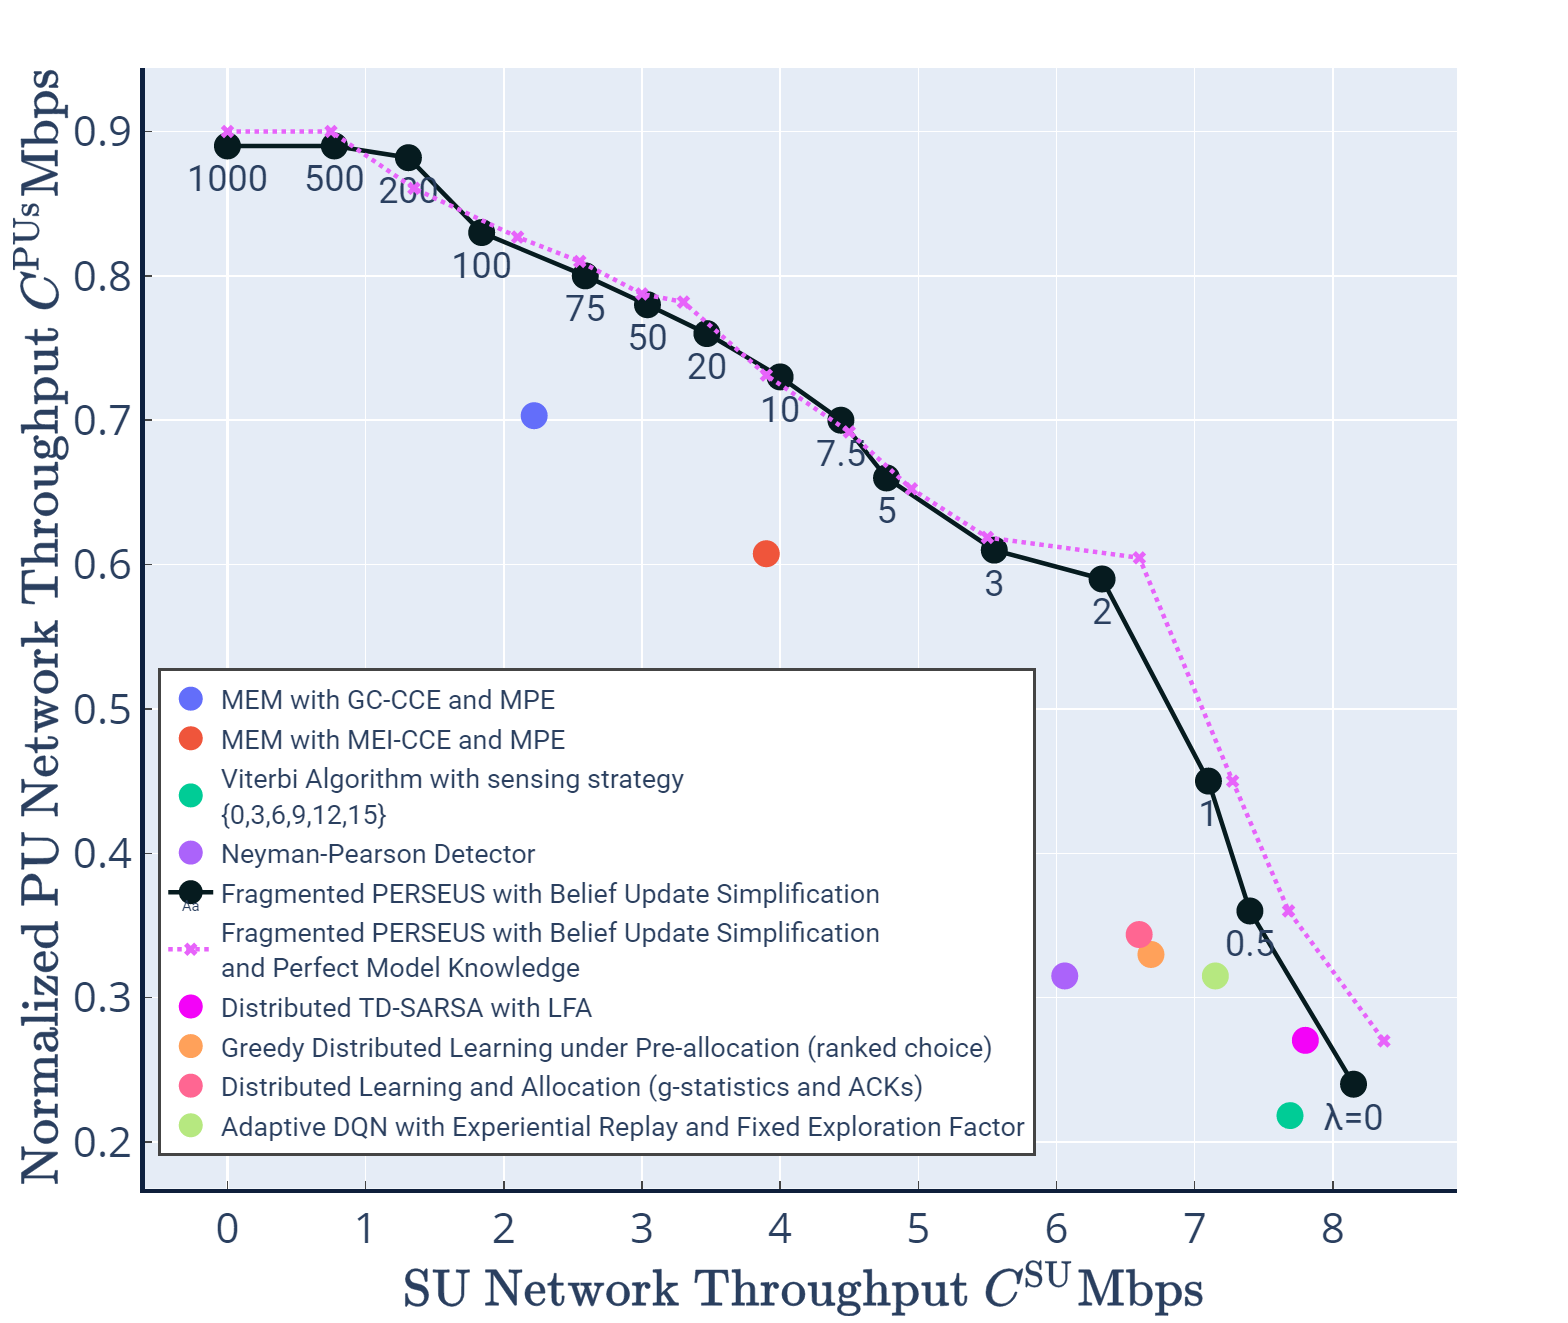
\includegraphics[width = 1.0\textwidth]{Throughput_and_Interference_with_DQN.png}}
    \caption{The evaluation of SU and PU network throughputs for different values of $\lambda$, along with comparisons with the state-of-the-art}
    \label{Fig. 4}
\end{figure}

Incorporating a concurrent parameter estimator embedded into the fragmented PERSEUS algorithm (with belief update simplification\texttt{-{}-}the Hamming distance state filter), with an iterative publisher-subscriber routine described in Section \ref{II.I}, we find that our framework outperforms the state-of-the-art algorithms that also tackle the spectrum sensing and access problem in a correlated incumbent occupancy behavior setting. Specifically, evaluating the performance of our framework against the Minimum Entropy Merging (MEM) algorithm with Greedy Clustering based Channel Correlation Estimation (GC-CCE) and Markov Process Estimation (MPE) \cite{WCL:7}, we find that with a correlation threshold of $\rho_{th}{=}0.77$ in the MEM with GC-CCE and MPE solution, our framework achieves a $104$\% improvement in the throughput attained by the SU, for the same level of interference to the incumbents in the network. Similarly, we find that our solution achieves a $38$\% improvement in the SU throughput, for the same level of PU interference, over the Minimum Entropy Merging (MEM) algorithm with Minimum Entropy Increment (MEI) Clustering based Channel Correlation Estimation (CCE) and Markov Process Estimation (MPE) with a correlation threshold of $\rho_{th}{=}0.77$ \cite{WCL:7}. Additionally, our solution attains a $25$\% increase in SU network throughput, for the same level of interference caused to the PUs in the network, over a Neyman-Pearson Detector that assumes independence among the channels across both frequency and time, has no channel sensing restrictions, involves an AND fusion rule across 300 different samplings, and whose threshold is determined based off of a specified false alarm probability of $0.3$ \cite{WCL:paper, WCL:11}. Finally, comparing the performance of our POMDP framework against well-known HMM state estimators\texttt{-{}-}specifically, the Viterbi algorithm that solves the MAP state estimation problem for the system described in this simulation setup consisting of a two chain Markovian correlation structure (one across time and the other across frequency) \cite{WCL:6}, with the same channel sensing restriction as ours, i.e., $6$, but that which knows the exact underlying MDP transition model $\mathbf{A}$ as an apriori, we note that our solution offers a $6$\% increase in the attained SU network throughput, for the same amount of incumbent interference. Sticking to the fact that our framework does not know the underlying MDP transition model\texttt{-{}-}which is governed by the correlated PU occupancy behavior\texttt{-{}-}ahead of time, but instead learns this correlation structure as it is interacting with the radio environment and solving for the optimal policy, we evaluated the accuracy of our optimal policy's behavior against a similar PERSEUS agent which knew the transition model beforehand: we find that in the worst-case with respect to the difference in performance between the two, i.e., when $\lambda{=}0$, for the same level of incumbent interference, knowing the correlation model ahead of time only provided a $3.75$\% increase in the attained SU network throughput\texttt{-{}-}which is a testament to the accuracy of our embedded parameter estimator and the iterative publish-subscribe to-and-fro between the EM thread and the PERSEUS thread. These evaluations are illustrated in Fig. \ref{Fig. 4}.
\begin{figure} [htb]
    \centerline{
    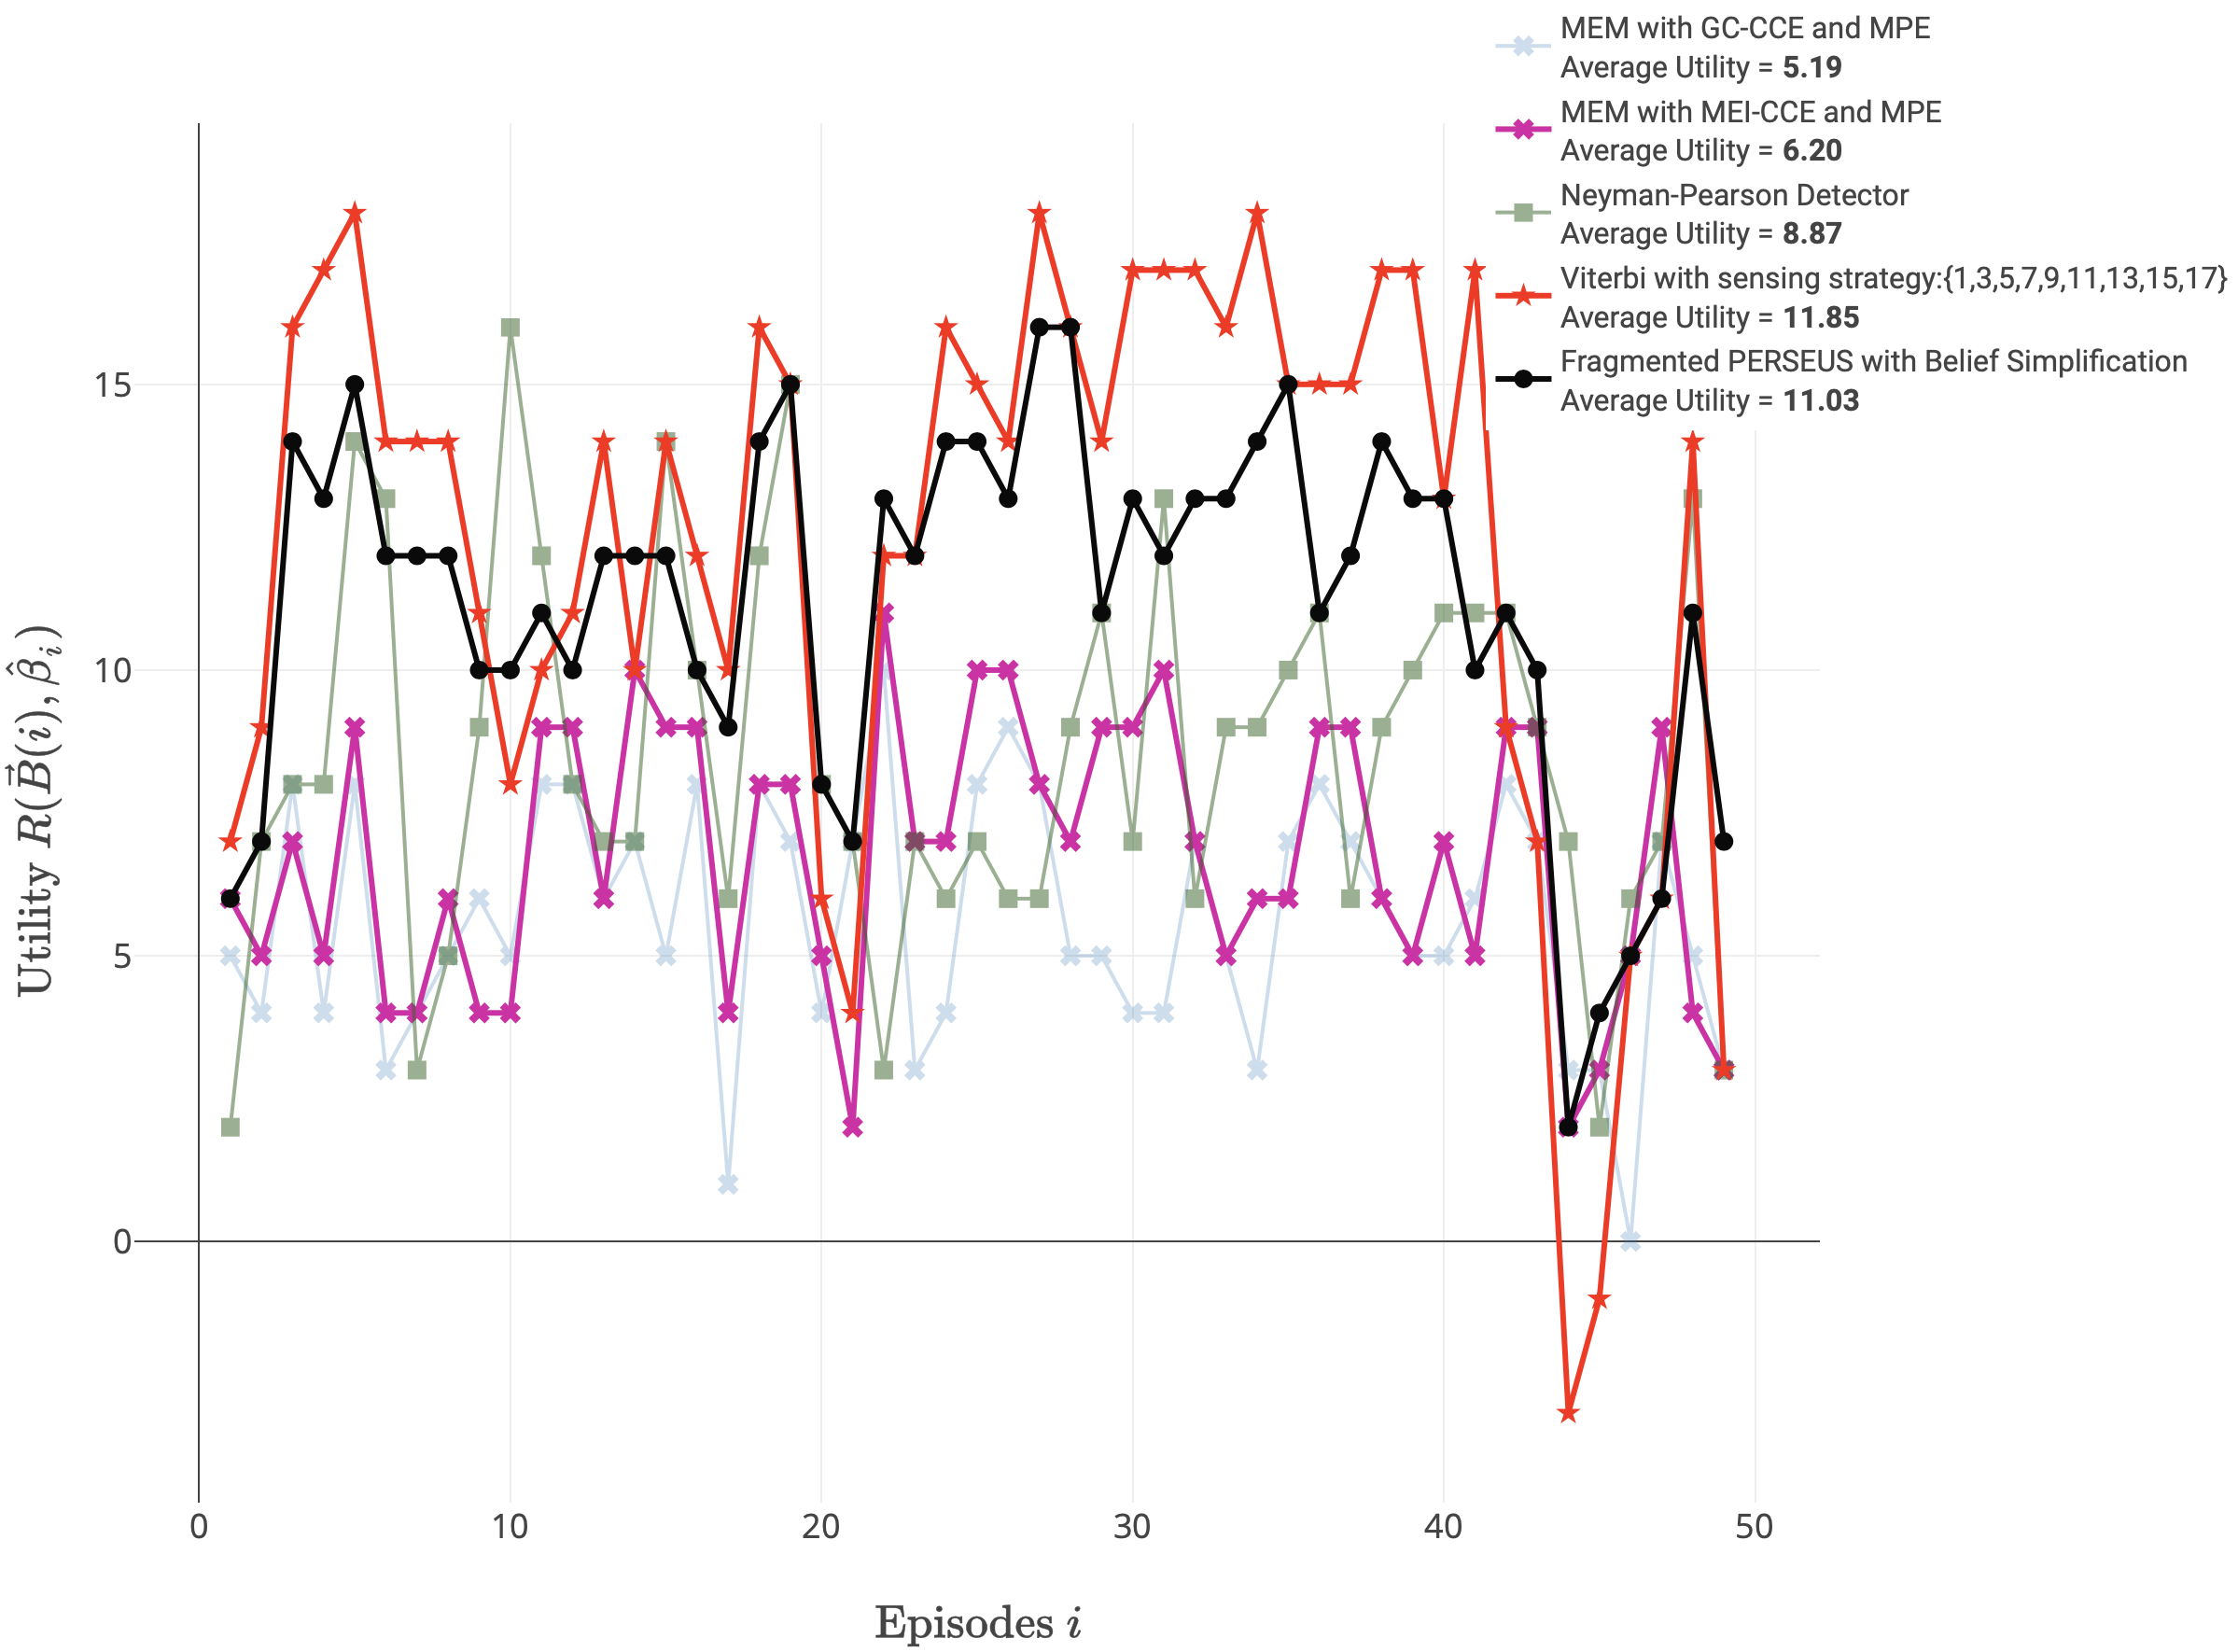
\includegraphics[width = 1.0\textwidth]{PerformanceEvaluation.png}}
    \caption{The evaluation of the proposed solution, from an average utility per time-slot perspective, against a medley of approaches in the state-of-the-art}
    \label{Fig. 5}
\end{figure}

Analyzing the performance of our POMDP solution from a different perspective, we find that, as illustrated in Fig. \ref{Fig. 5}, our framework obtains an average utility, i.e., $R(\vec{B}(i),\hat{\beta}_{i})$ described in Section \ref{I.IV}, of $11.03$ per time-step $i$\texttt{-{}-} $112$\% higher than that achieved by the MEM with GC-CCE and MPE algorithm from \cite{WCL:7}, $80$\% higher than that achieved by the MEM with MEI-CCE and MPE algorithm from \cite{WCL:7}, and $25$\% more than that attained by the Neyman-Pearson Detector detailed above \cite{WCL:11}. Furthermore, in order to understand how our framework performs against a standard HMM state estimation solution like the Viterbi algorithm described earlier \cite{WCL:6}\texttt{-{}-}especially, one with apriori transition model information and one that senses a maximum of $9$ channels as opposed to our $6$ (in order to contrast this with the previous comparison with the Viterbi algorithm in which both have the same channel sensing restrictions)\texttt{-{}-}we compare our solution with this Viterbi agent, and find that in spite of this Viterbi agent having more occupancy information per time-step (owing to it sensing a maximum of $3$ additional channels), the average utility obtained by the Viterbi agent (${=}11.85$) is only $7$\% higher than ours (${=}11.03$).
\begin{figure} [htb]
    \centerline{
    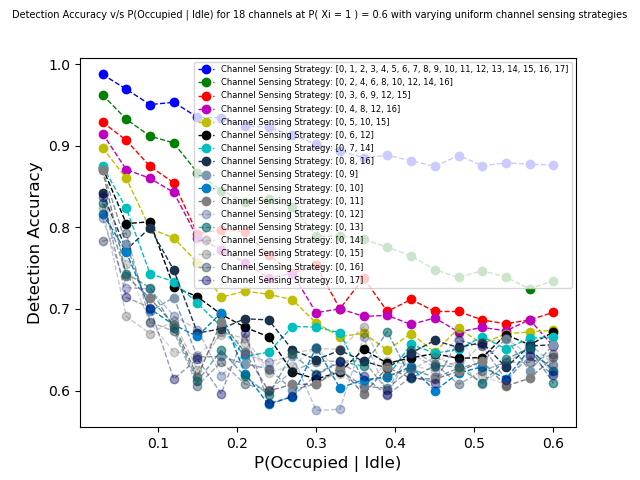
\includegraphics[width = 1.0\textwidth]{Uniform_Channel_Sensing.png}}
    \caption{The evaluation of estimation accuracies for different channel sensing strategies, corresponding to a single frequency-correlation Markov chain Viterbi algorithm, in relation to variations in the amount of correlation}
    \label{Fig. 6}
\end{figure}

As opposed to the double-chain Viterbi algorithm described above, now we separately simulate a single-chain Viterbi algorithm to address the advantage of having more sensing information and to prove a few results about the importance of leveraging the correlations in incumbent occupancy behavior across frequencies, which many works in the state-of-the-art fail to do. Addressing the advantage of having more sensing information, Fig. \ref{Fig. 6} drives home the point that sensing more channels improves the accuracy of the HMM state estimator, i.e., the Viterbi algorithm discussed here, which in turn gives the SU a better occupancy picture, and hence, a higher average utility per time-step for the Viterbi algorithm over ours, as seen in Fig. \ref{Fig. 5}. As we go down the plot in Fig. \ref{Fig. 6}, i.e., as the number of channels sensed per time-step decreases, the estimation accuracy/detection accuracy, which refers to the number of channels whose states ($0$ or $1$) were correctly estimated by the Viterbi algorithm\texttt{-{}-}mathematically described as $\sum_{k{=}1}^{K}\mathcal{L}\left\{B_{k}(i){=}\hat{B}_{k}(i)\right\}$, where $\mathcal{L}$ is an indicator variable, $B_{k}(i){\in}\{0,1\}$ is the true occupancy state of the channel in time-slot $i$, and $\hat{B}_{k}(i){\in}\{0,1\}$ is the occupancy state of the channel estimated by the Viterbi algorithm\texttt{-{}-}averaged over $300$ sampling rounds, decreases consistently.

Two additional points about the effects of correlation in incumbent occupancy behavior across frequency on the accuracy of state estimation can be made by analyzing Fig. \ref{Fig. 6} from a different perspective\texttt{-{}-}the first being that as the incumbent occupancy behavior becomes more and more correlated across frequency, as denoted by the X-axis, i.e., as $\mathbb{P}(B_{k+1}(i){=}1|B_{k}(i){=}0),{\forall}1{\leq}k{\leq}K$ moves from a highly correlated model ($\mathbb{P}(B_{k+1}(i){=}1|B_{k}(i){=}0){=}0.1{>}0.6{=}\mathbb{P}(B_{k+1}(i){=}1),{\forall}1{\leq}k{\leq}K$) to an independence model ($\mathbb{P}(B_{k+1}(i){=}1|B_{k}(i){=}0){=}0.6{=}\mathbb{P}(B_{k+1}(i){=}1),{\forall}1{\leq}k{\leq}K$), the estimation accuracy/detection accuracy decreases; and the second point being that as the gap between the consecutive channels sensed by the agent increases, the estimation/detection accuracy worsens\texttt{-{}-}as evident from the final few plot lines in Fig. \ref{Fig. 6}\texttt{-{}-}for instance, the estimation accuracy for channel sensing strategy $[0,9]$ is higher than that for strategy $[0,17]$, for the same amount of PU occupancy correlation across frequency ($\mathbb{P}(B_{k+1}(i){=}1|B_{k}(i){=}0){=}0.1,{\forall}1{\leq}k{\leq}K$). Therefore, this evaluation of the single-chain Viterbi algorithm in a separate, hypothetical simulation model proves that we can achieve  an improved estimation of incumbent occupancy behavior by sensing more channels per time-step and by leveraging the correlations in PU occupancy behavior across frequencies. However, as already noted, the number of channels that can be simultaneously sensed by the SU in a given time-step is restricted by design limitation \cite{WCL:3}\texttt{-{}-}hence, fixing $\kappa{=}6$ in our POMDP solution, we resort to leveraging the correlation in incumbent occupancy behavior across frequency (and time) in order to attain better performance. Additionally, we find that adapting the spectrum sensing decision based on the system state (true or perceived) \cite{WCL:paper, WCL:5}, in contrast to a fixed sensing strategy \cite{WCL:6, WCL:7}, adds to the performance gains attained by exploiting the PU occupancy correlation.

As already discussed, our proposed framework can be decomposed into two components: the parameter estimator and PERSEUS. Next, we take up each of these two individually and analyze their performance.
\begin{figure} [htb]
    \centerline{
    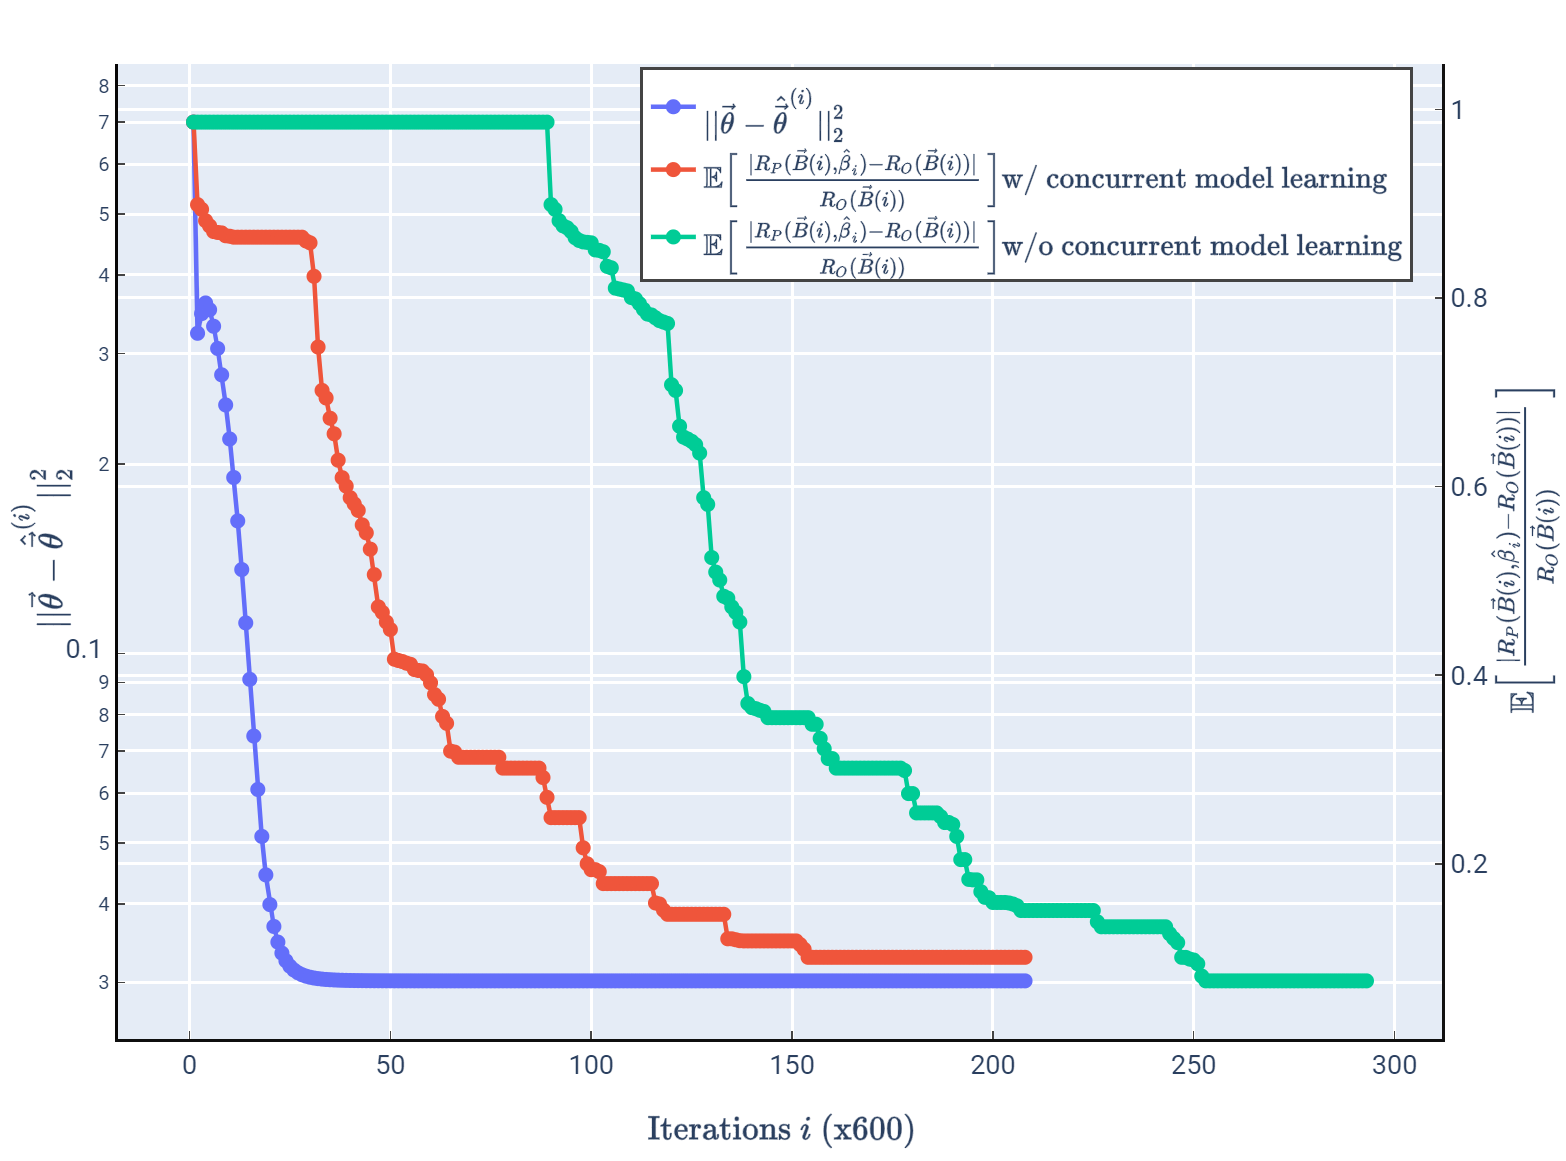
\includegraphics[width = 1.0\textwidth]{HMM_EM_Speed_Up.PNG}}
    \caption{The convergence of the MSE of the HMM EM algorithm to estimate $\vec{\theta}$, and the convergence of the loss of the fragmented PERSEUS algorithm with belief update simplification}
    \label{Fig. 7}
\end{figure}

Specifically discussing the performance of the parameter estimation algorithm, i.e., the EM algorithm, we find that, with initial estimates of $0.5$, i.e., $p_{uv}{=}0.5,{\forall}u,v{\in}\{0,1\}$ and $q_{w}{=}0.5,w{\in}\{0,1\}$, the estimator converges to the true parameter vector $\vec{\theta}$ with an error/delta of $\eta{=}10^{-8}$ in $45,000$ iterations\texttt{-{}-}this corresponds to an observation and estimation period of $135$s, considering a typical time-slot duration of $3$ms \cite{WCL:paper}. We illustrate this convergence via the Mean Square Error (MSE) plot depicted in Fig. \ref{Fig. 7}, in which the MSE in iteration $t$ given by,
\begin{equation}\label{32}
    ||\vec{\theta}-\hat{\vec{\theta}}^{(t)}||_{2}^{2}=\sum_{\theta \in \vec{\theta}}\mathbb{E}[(\theta-\hat{\theta}^{(t)})^{2}]
\end{equation}
is decreased iteratively, as the estimation process goes through the E-step and the M-step in each iteration $t$ until $\mathbb{E}[\theta{-}\hat{\theta}^{(t)}]{\leq}10^{-8},{\forall}\theta{\in}\vec{\theta}$.

On the same time-scale as the parameter estimation algorithm, focusing on the loss convergence of the PERSEUS algorithm with a discount factor of $\gamma{=}0.9$ and a termination threshold of $\epsilon{=}10^{-5}$, wherein we define the expected loss as the difference between the utility obtained by the proposed PERSEUS framework, denoted by $R_{P}(\vec{B}(i))$ (discussed in Section \ref{I.IV}), and that obtained by an Oracle, which knows the exact occupancy behavior of the incumbents in the network, denoted by $R_{O}(\vec{B}(i))$\texttt{-{}-}we find that, as depicted in Fig. \ref{Fig. 7}, the loss convergence of PERSEUS is relatively slower while the parameter estimator is learning the transition model; as opposed to after the convergence of the parameter estimator, when we see a more consistent gradient towards the optimality.

Finally, inspecting Fig. \ref{Fig. 4} in a new light, we see that our POMDP agent limits channel access when the penalty ($\lambda$) is high\texttt{-{}-}leading to lower SU throughput and lower PU interference\texttt{-{}-}and conversely, follows a more lenient channel access strategy when the penalty is low\texttt{-{}-}resulting in higher SU throughput and higher PU interference. Generally speaking, Fig. \ref{Fig. 4} depicts a trend of increasing SU throughput and increasing incumbent interference, as the penalty for missed detections, i.e., $\lambda$ is lowered \cite{WCL:paper}. Therefore, our framework provides a crucial practical tool in cognitive radio MAC design\texttt{-}the ability to tune the trade-off between the throughput obtained by the cognitive radio and the interference caused by it to incumbent transmissions in the network.

\section{Feasibility Analysis of the POMDP Optimal Policy on ESP32 Radios}\label{D}
\begin{figure} [htb]
    \centerline{
    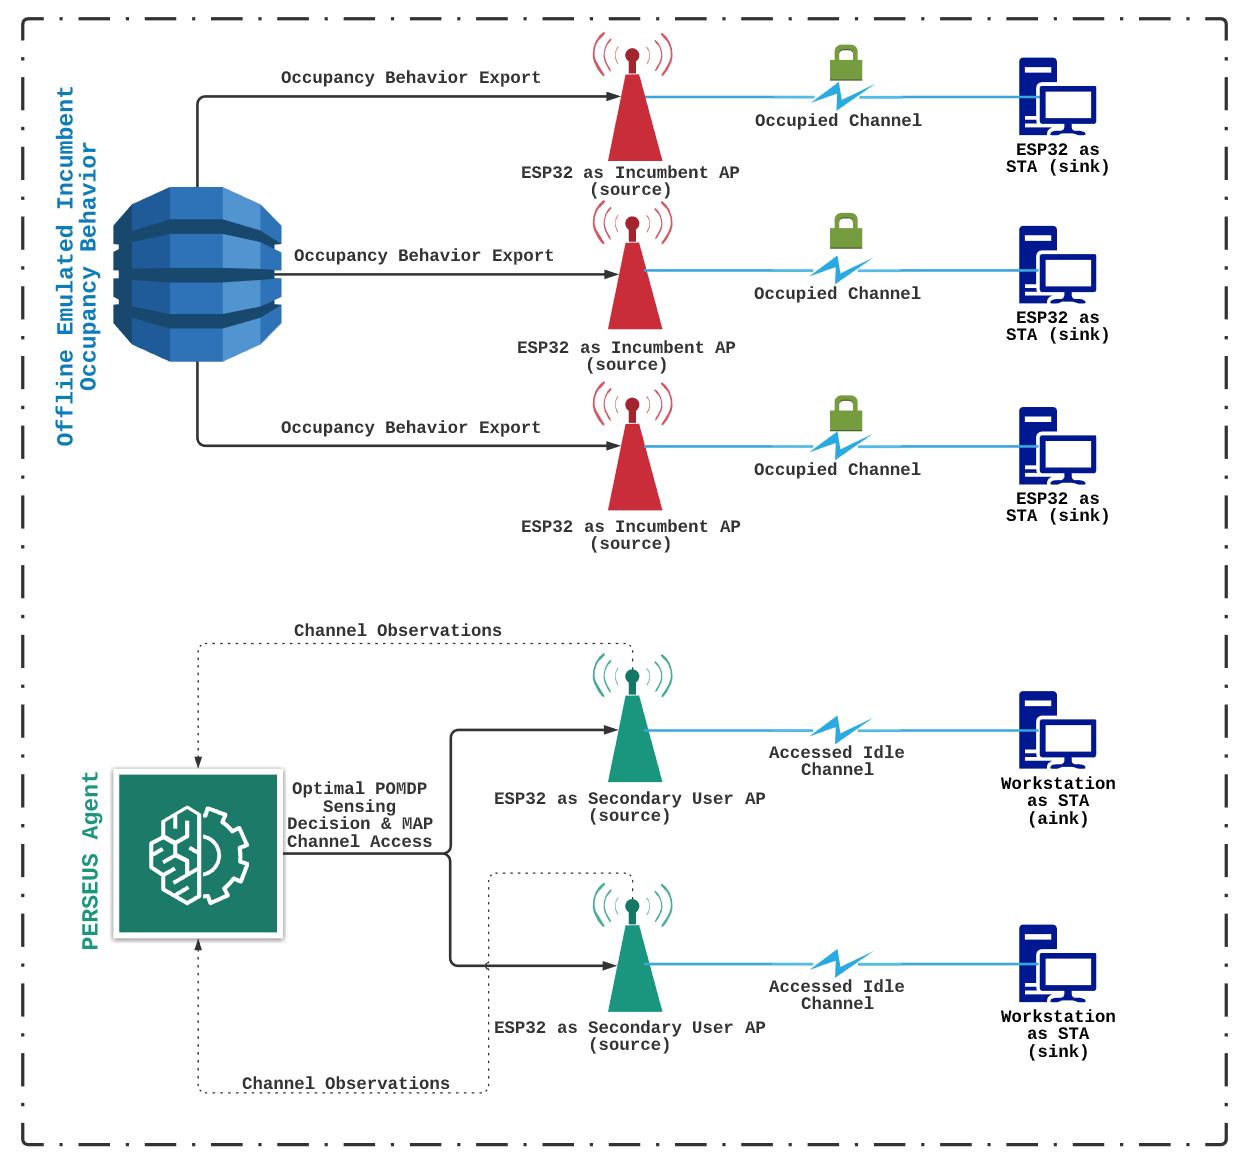
\includegraphics[width = 1.0\textwidth]{Minerva_ESP32_Deployment_Model.png}}
    \caption{The deployment setup of a distributed ad-hoc WLAN network for feasibility analysis of the PERSEUS optimal policy}
    \label{fig: C. 0}
\end{figure}
We employ $8$ ESP32 radios \cite{Espressif:ESP32}, with each one embedded in a GCTronic e-puck2 robot \cite{GCTronic:epuck2}, categorized into a network of $3$ PUs (and their $3$ corresponding sinks) occupying $6$ channels in the discretized spectrum of interest according to a Markovian time-frequency correlation structure (described by \eqref{6})\texttt{-{}-}and $2$ independent SUs, with each having the capability of sensing only one channel at a time, intelligently trying to exploit the white-spaces in the spectrum. The detailed methodology of this implementation is provided below:
\begin{enumerate}
    \item Considering a network with $J{=}3$ PUs and one SU with a channel sensing restriction of $\kappa{=}2$ out of $K{=}6$ channels in the discretized spectrum of interest\texttt{-{}-}and assuming a linear AWGN observation model, with a Rayleigh channel fading model (discussed in Section \ref{I.I}), we simulate the occupancy behavior of the PUs according to a Markovian time-frequency correlation structure parameterized by $\vec{\theta}{=}[\vec{p},\vec{q}]^{\intercal}$, where $\vec{p}{=}[p_{00}{=}0.1,p_{01}{=}0.3,p_{10}{=}0.3,p_{11}{=}0.7]^{\intercal}$ and $\vec{q}{=}[q_{0}{=}0.3,q_{1}{=}0.8]^{\intercal}$; and solve for the optimal spectrum sensing and access policy using PERSEUS, embedded with a concurrent parameter estimation algorithm learning the parameter vector $\vec{\theta}$\texttt{-{}-}by mimicking the observational capabilities of the actual ESP32 radios. Note this step is performed on a PC.
    \item The simulated PU occupancy behavior\texttt{-{}-}Markovian correlated according to \eqref{6} and parameterized by $\vec{\theta}$, and the time-slot specific optimal channel access decisions (derived off of the POMDP optimal sensing policy and the simulated PU occupancy behavior), are stored in databases (for export onto the ESP32 network).
    \item Peer-to-Peer communication links are established between a PU ESP32 radio and its sink, using the $3$ ESP32 radios designated as PUs\texttt{-{}-}in other words, $3$ wireless communication links are established: one for each ESP32 PU pair (a source and a sink), over WiFi ($2.4$GHz) and using a channel according to the occupancy information detailed in the exported PU occupancy database, in time-slot $i$.
    \item Note here that in this ESP32 PU network implementation, in time-slot $i$, while establishing a wireless communication link between a ESP32 PU $j{\in}\{1,2,3\}$ and its respective sink $i{\in}\{1,2,3\}\text{ s.t.}i\text{ is the designated sink for PU}j$, i.e., while forming link $l_{ij}$ over channel $k_{l_{ij}}{=}k{\in}\{1,2,\dots,6\}$ (as determined by the exported PU occupancy database which contains simulated PU occupancy behavior according to the Markovian time-frequency correlation structure described above) such that $k_{l_{ij}}{\neq}k_{l_{i',j'}},{\forall}i,i'{\in}\{1,2,3\},j,j'{\in}\{1,2,3\}$\texttt{-{}-}PU $j$ serves as an Access Point (AP) accepting transmission requests from PU $i$, which is designates as a STAtion (STA). In the next synchronized time-slot $i+1$, this link $l_{ij}$ moves to channel $k'{\in}\{1,2,\dots,6\}$, as detailed in the exported PU occupancy database. This same procedure takes place for the other two incumbent communication links in every time-slot until the end of the implementation evaluation period.
    \item Although the PC-based POMDP solver employs an SU which can access $2$ channels at a time in order to deliver its flows (see the access part of the POMDP formulation in Section \ref{I.IV}), we employ $2$ ESP32 SU radios in the network\texttt{-{}-}with the channel access work synchronously and evenly split between the two\texttt{-{}-}due to the actual physical design limitation of the ESP32 radio that a it can only access one channel at a time, forcing us to be creative: split the optimal $2$ channel access decision in time-slot $i$, as determined by the time-slot specific optimal POMDP channel access database, into a single-channel access action at each ESP32 SU radio. Next, based on whether the channel access at the $2$ ESP32 SU radios was successful, we compute the success rate.
\end{enumerate}
The deployment setup of this distributed ad-hoc WLAN network\texttt{-{}-}for evaluating the implementation feasibility of the POMDP optimal policy\texttt{-{}-}is illustrated in Fig. \ref{fig: C. 0}.
\section{Implementation Results}\label{D.I}
The channel access success rate metric defined as
\begin{equation}\label{C.I}
    \text{Channel Access Success Probability}=\frac{\sum_{j=1}^{2}\mathcal{I}\left\{B_{k_{SU_{j}}}(i)=0\right\}}{2},
\end{equation}
where $\mathcal{I}$ corresponding to $\mathcal{I}\left\{B_{k_{SU_{j}}}(i)=0\right\}$ is an indicator variable whose value is $1$ if the channel accessed by the ESP32 SU $j{\in}\{1,2\}$ in time-slot $i$ is not occupied by an incumbent PU ESP32 radio, and $B_{k_{SU_{j}}}{\in}\{0,1\}$ is the occupancy variable of the channel accessed by the ESP32 SU $j$ in time-slot $i$\texttt{-{}-}is evaluated per time-slot $i$, and the resultant metrics are plotted against time, which is illustrated in Fig. \ref{fig:C.1}.
\begin{figure} [htb]
    \centerline{
    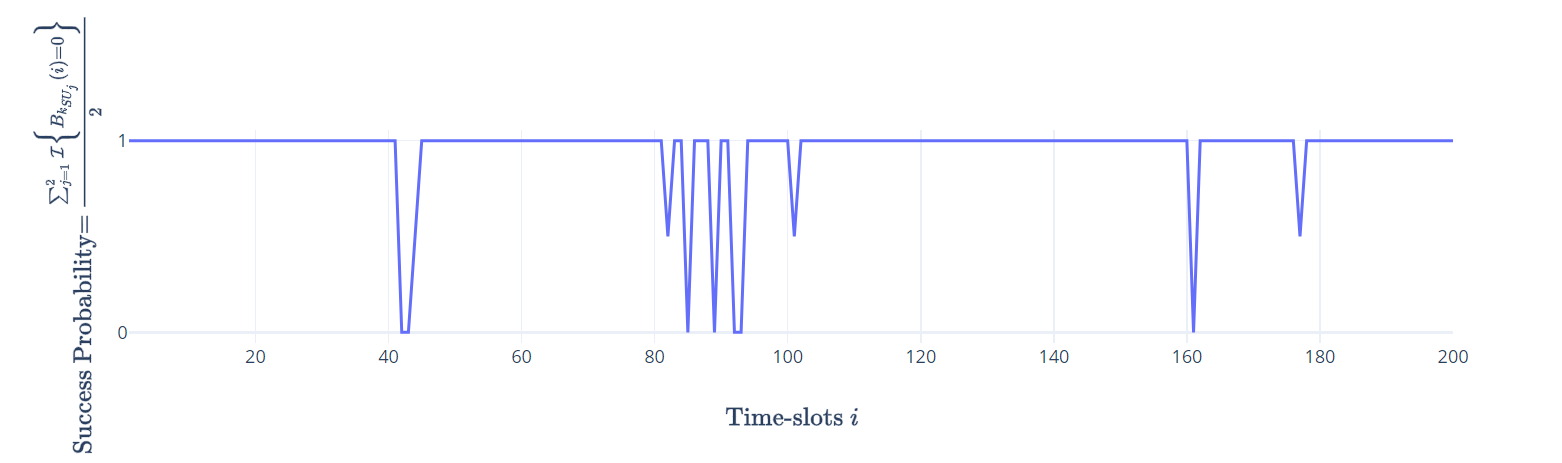
\includegraphics[width = 1.0\textwidth]{ESP32_Success_Probability.PNG}}
    \caption{The channel access probability of the ESP32 SU radios per time-slot}
    \label{fig:C.1}
\end{figure}
\section{Conclusion}\label{V}
In this letter, we formulate the optimal spectrum sensing and access problem in cognitive radio networks via POMDPs. In a radio environment wherein the occupancy behavior of the incumbents is correlated across time and frequencies, we present a framework that employs the EM algorithm to estimate the transition model of this occupancy behavior, and leverage a fragmented PERSEUS algorithm with belief update heuristics to concurrently solve for the optimal spectrum sensing and access policy. In addition to its superior performance compared to the state-of-the-art, our framework facilitates regulation of the trade-off between SU throughput and PU interference.
\bibliographystyle{IEEEtran}
\bibliography{ref}
\end{document}